\documentclass[letterpaper,10pt,conference]{IEEEtran} % Comment if a4paper
% \documentclass[a4paper,10pt,conference]{IEEEtran}   % Uncomment for a4 paper
\IEEEoverridecommandlockouts                          % Only needed if you want to use the \thanks command (funding)

% TEMPLATE VERSION DATA: 27/06/2024

\usepackage{cite}     % compressed, sorted lists of numerical citations
\usepackage{hyperref} % cross-referencing to generate hyperlints in the document
\usepackage{amsmath}  % enhanced functions to improve math content display
\usepackage{amssymb}  % math symbols
\usepackage{amsfonts} % math extended fonts
\usepackage{graphicx} % enhanced support for graphics display
\usepackage[font=small]{caption}
\usepackage[font=footnotesize]{subcaption}
\usepackage{algorithmicx}         % pseudocode environments
\usepackage[noend]{algpseudocode}
\usepackage{enumitem} % control layout of itemize, enumerate, description
\usepackage{svg}      % include svg graphics
\usepackage{textcomp} % additional text symbols (e.g., bullet, copyright, ...)
\usepackage{xcolor}   % color extensions

% \usepackage[backend=biber,
%             %style=apa,
%             %style=numeric,
%             style=numeric-comp,
%             bibstyle=numeric,
%             %citestyle=authoryear-comp,
%             citestyle=numeric-comp,
%             %sorting=nyt,
%             sorting=none,
%             maxnames=8,
%             minnames=3
%             %maxcitenames=2,
%             %mincitenames=1
%             ]{biblatex}

%% Style hacks to save space
% \setlength{\textfloatsep}{1.5em}
% \setlength{\dbltextfloatsep}{1.5em}

%% Key definitions for text elements.
\def\secref#1{Section~\ref{#1}}
\def\figref#1{Fig.~\ref{#1}}
\def\tabref#1{Table~\ref{#1}}
\def\eqref#1{Equation~(\ref{#1})}
\def\algref#1{Algorithm~\ref{#1}}

%% Other useful macros
\newcommand\todo[1]{\textbf{[TODO: #1}]}
\newcommand\etal{\emph{et~al.}}

%% Some math definition
\def\argmax{\mathop{\rm argmax}}
\def\argmin{\mathop{\rm argmin}}
\newcommand{\bigO}[1]{$\mathcal{O}(#1)$}

\thispagestyle{empty}
\pagestyle{empty}

%% Bibliography (biblatex)
% \addbibresource{references.bib}
% \renewcommand*{\bibfont}{\normalfont\small}



%%%%%%%%%%%%%%%%%%%%%%%%%%%%%%%%%%%%%%%%%%%%%%%%%%%%%%%%%%%%%%%%%%%%%%%%%%%%%%%%



\def\finalversion{}
% \let\finalversion\undefined



%%%%%%%%%%%%%%%%%%%%%%%%%%%%%%%%%%%%%%%%%%%%%%%%%%%%%%%%%%%%%%%%%%%%%%%%%%%%%%%%



\begin{document}

\bstctlcite{IEEEexample:BSTcontrol}

\title{Integrating Multimodal Perception into\\Ground Mobile Robots
\thanks{%
\ifdefined\finalversion%
This work is co-financed by Component 5 -- Capitalization and Business
Innovation, integrated in the Resilience Dimension of the Recovery and
Resilience Plan within the scope of the Recovery and Resilience
Mechanism~(MRR) of the European Union~(EU), framed in the Next~Generation~EU,
for the period 2021--2026, within project GreenAuto, with reference 54.
\else%
Removed for blind revision.%
\fi%
}%
}

\author{%
%
\ifdefined\finalversion%
%
\IEEEauthorblockN{%
Ricardo B. Sousa\IEEEauthorrefmark{1}\IEEEauthorrefmark{2},
H\'{e}ber Miguel Sobreira\IEEEauthorrefmark{2},
Jo\~{a}o G. Martins\IEEEauthorrefmark{1}\IEEEauthorrefmark{2},\\%
Paulo G. Costa\IEEEauthorrefmark{1}\IEEEauthorrefmark{2},
Manuel F. Silva\IEEEauthorrefmark{2}\IEEEauthorrefmark{3}, and
Ant\'{o}nio Paulo Moreira\IEEEauthorrefmark{1}\IEEEauthorrefmark{2}}%
%
\IEEEauthorblockA{%
\IEEEauthorrefmark{1}Faculty of Engineering, University of Porto (FEUP), 4200-465 Porto, Portugal.
\{\href{mailto:rbs@fe.up.pt}{rbs},%
\href{mailto:paco@fe.up.pt}{paco},%
\href{mailto:amoreira@fe.up.pt}{amoreira}\}@fe.up.pt}%
%
\IEEEauthorblockA{%
\IEEEauthorrefmark{2}INESC TEC -- Institute for Systems and Computer Engineering,
Technology and Science, 4200-465 Porto, Portugal.\\%
\{\href{mailto:heber.m.sobreira@inesctec.pt}{heber.m.sobreira},%
\href{mailto:joao.g.martins@inesctec.pt}{joao.g.martins}\}@inesctec.pt}%
%
\IEEEauthorblockA{%
\IEEEauthorrefmark{3}ISEP, Polytechnic of Porto, 4249-015 Porto, Portugal.
\href{mailto:mss@isep.ipp.pt}{mss@isep.ipp.pt}}%
\else%
%
Removed for blind revision.%
\fi%
}

\maketitle



%%%%%%%%%%%%%%%%%%%%%%%%%%%%%%%%%%%%%%%%%%%%%%%%%%%%%%%%%%%%%%%%%%%%%%%%%%%%%%%%



\begin{abstract}
%% WHY is it relevant?
% \emph{1-2 not too long sentences clearly answering the WHY question.}
%% WHICH PROBLEM do we address?
% In this paper, we address the problem of ...
%% HOW is our approach special, WHAT are we actually doing, and WHAT IS NEW
% Our approach ... \emph{(complete, around 2-3 sentences)}
%% IMPLEMENTATION, EVALUATION, WHAT FOLLOWS FROM IT
% We implemented our approach using C++ and ROS and thoroughly tested
% it on .... \emph{(finish sentence)}. The experiments presented in
% this paper suggest that ... \emph{(finish sentence)}

Multimodal perception systems enhance the robustness and adaptability
of autonomous mobile robots by integrating heterogeneous sensor modalities,
improving long-term localisation and mapping in dynamic environments and
human-robot interaction. Current mobile platforms often focus on specific
sensor configurations and prioritise cost-effectiveness, possibly limiting
the flexibility of the user to extend the original robots further.
This paper presents a methodology to integrate multimodal perception into a
ground mobile platform, incorporating wheel odometry, 2D~laser scanners,
3D~Light Detection and Ranging (LiDAR), and RGBD cameras.
The methodology describes the electronics design to power devices, firmware,
computation and networking architecture aspects, and mechanical mounting
for the sensory system based on 3D~printing, laser cutting, and
bending metal sheet processes. Experiments demonstrate the usage of the
revised platform in 2D and 3D~localisation and mapping and pallet pocket
estimation applications. All the documentation and designs are accessible
in a public repository.
\end{abstract}

\begin{IEEEkeywords}
Light Detection and Ranging (LiDAR), mobile robot, multimodal perception, open-source, RGBD camera.
\end{IEEEkeywords}



%%%%%%%%%%%%%%%%%%%%%%%%%%%%%%%%%%%%%%%%%%%%%%%%%%%%%%%%%%%%%%%%%%%%%%%%%%%%%%%%



\section{Introduction}\label{sec:intro}

%% WHY
% WHY: First, answer the WHY question. Why is that relevant? Why should I be
% motivated to read the paper?
%% WHICH PROBLEM
% WHICH PROBLEM: Second, explain WHICH problem you are solving/address to solve.
%% HOW & WHAT
% HOW \& WHAT: Third, explain briefly how one can address/model/solve the
% problem and mention briefly what others/we before have done. Prepare the
% reader for your contribution that comes in the next section.
% Motivating Example. Provide a caption that lets the reader understand
% the image easily.  This image should be on top of the right column of page 1.
%% MAIN CONTRIBUTION & WHAT FOLLOWS FROM THAT
% Explain your contribution in one paragraph. Start that paragraph with:
% The main contribution of this paper is a ...  We achieve this by
% ... This allows us to ... See \figref{fig:motivation} for an example.
%% CLAIMS (can be merged with the main contribution above)
% Claims: Explicitly state your claims in one (short) paragraph. For example:
% In sum, we make four key claims:
% Our approach is able to
% %
% (i) ...,
% %
% (ii) ...,
% %
% (iii) ... and,
% %
% (iv) .
% %
% These claims are backed up by the paper and our experimental evaluation.

Multimodal perception systems pose unique challenges for
autonomous mobile robots, requiring the real-time integration of
asynchronous and heterogeneous data streams.
These systems provide rich information, enabling robust interactions
between humans and robots~\cite{duncan2024jhri}.
Another advantage of multimodal perception is enhancing the
robustness of localisation and mapping algorithms,
particularly in long-term applications with
scene appearance changes~\cite{sousa2023jfr}.

As a result, integrating multimodal perception into ground mobile platforms
improves the robustness of autonomous systems by
combining diverse sensor modalities.
This integration requires the consideration of several factors,
including mechanical mounting, electronics design to power the sensors,
and the computing architecture to gather and process sensor data.
Currently, most commercially available and research-oriented mobile platforms
focus on specific sensor models. These platforms typically prioritise
low-cost solutions or have multimodal perception with a
particular sensor configuration.

\begin{figure}[t]
\centering
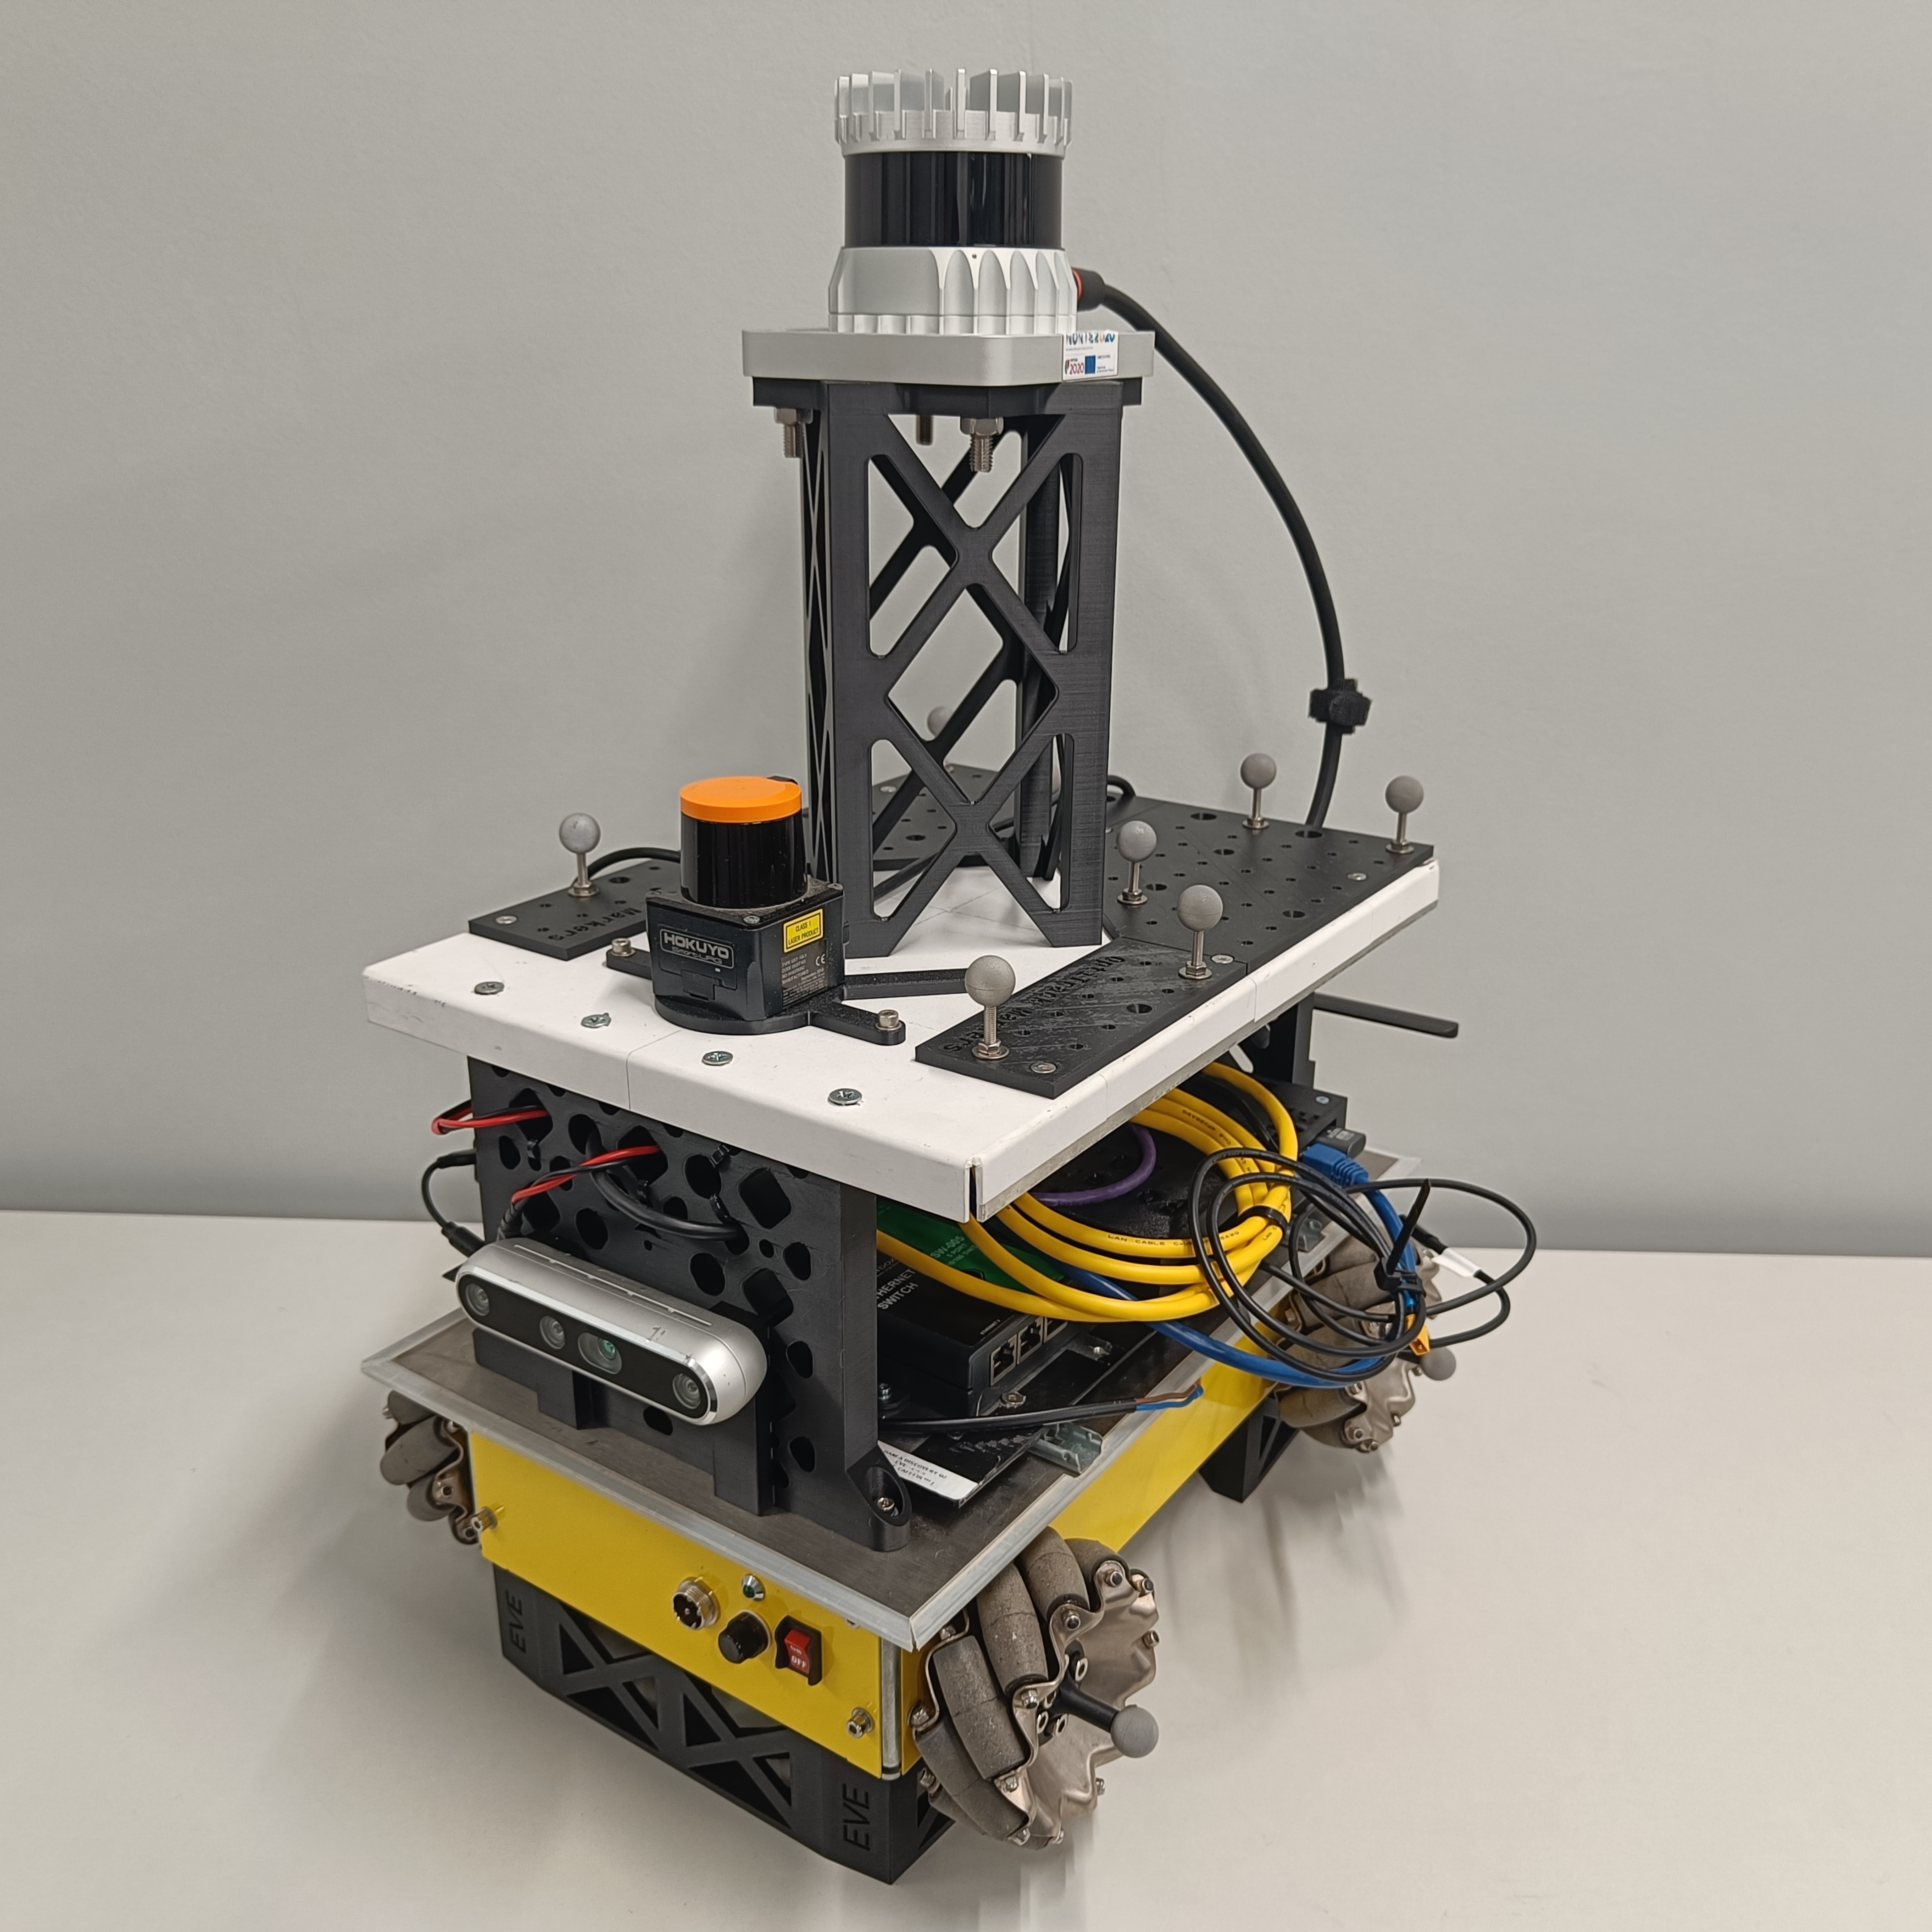
\includegraphics[width=0.5\columnwidth]{figs/hangfa-discovery-q2_revised-platform_photo_perspective_square.jpg}
\caption{Revised Hangfa Discovery~Q2
mobile platform
with multimodal perception
(2D laser scanner -- Hokuyo UST-10LX; 3D LiDAR -- Ouster OS1~64;
and RGBD camera -- Intel RealSense~D455).}
\label{fig:hangfa:revised-platform}
\end{figure}

This paper outlines a methodology to integrate multimodal perception
into a ground mobile robot. The multimodal system incorporates
2D laser scanners, 3D Light Detection and Ranging (LiDAR), and
RGBD (colour and depth) sensors. This system includes
compatibility with at least four 2D lasers
(Hokuyo UST-10LX, LD-19, RPLIDAR~S2, and YDLIDAR~X4),
and several LiDARs (Livox~Mid-360, Ouster OS, RoboSense Helios,
Velodyne Puck/VLP) and RGBD camera
(Intel RealSense D455/455f/456/L515, OAK-D and OAD-D Pro Series) models.
The compatibility is achieved by relying on 3D printing and
bent metal sheet fabrication processes with laser-cut hole patterns
to standardise the sensor fixation onto the platform.
Furthermore, this paper details a comprehensive overhaul of an
omnidirectional platform, enabling wheel odometry,
the computing unit's integration onto the platform,
and defining a network architecture
for communication between sensors and other devices.
\figref{fig:hangfa:revised-platform} illustrates the
revised Discovery~Q2\footnote{\url{https://www.hangfa-europe.com/en/omni-robot/discovery}}
platform used to demonstrate the application of the
multimodal perception system.
Experiments include tests
on 2D and 3D Simultaneous Localisation and Mapping~(SLAM)
with 2D lasers and 3D LiDARs, and pallet pocket detection
with 2D~localisation and RGBD perception.

All electronics documentation,
mechanical designs for the bent metal sheets,
3D-printed components, and other parts,
along with the code developed in the scope of this paper,
are accessible in a public
\ifdefined\finalversion%
repository\footnote{\label{note:repo}\url{https://gitlab.inesctec.pt/mrdt/open-source/inesctec_mrdt_hangfa_discovery_q2}}.
\else%
repository\footnote{\label{note:repo}Removed for blind revision.}.
\fi
The repository aims to facilitate the replication of the
adaptations made to the original Hangfa Discovery~Q2 and
multimodal perception integration into the robot,
while also enabling the adaptation of this work to 
other ground mobile platforms and other applications.



%%%%%%%%%%%%%%%%%%%%%%%%%%%%%%%%%%%%%%%%%%%%%%%%%%%%%%%%%%%%%%%%%%%%%%%%%%%%%%%%



\section{Related Work}\label{sec:related}

% Discuss the main related work and cite around 12-20 papers in
%   sum. The related work section should be approx. 1 column long,
%   assuming a 6-page paper. Structure the section in paragraphs,
%   grouping the papers, and describing the key approaches with 1-2
%   sentences. If applicable, describe the key difference to your
%   approach at the end of each paragraph briefly. Avoid adding
%   subsections for a conference paper.
% Example text fragments:
% The approach by Stachniss \etal~\cite{stachniss2005aaai} aims at
% predicting ...
% Stachniss and Burgard~\cite{stachniss2005aaai} address the problem of dealing
% with...
% In contrast to that, Stachniss and Burgard~\cite{stachniss2005aaai}
% model different instances of typical world states using clustering.
% There are furthermore approaches that combine ....  at city
% scale~\cite{stachniss2005aaai}.
% If useful, BRIEFLY summarize your key contributions again at the
%   end, for example:
%   In this paper, we introduce a ... scheme that is
% inspired by the work of Stachniss \etal~\cite{stachniss2005aaai}
% but it extends the original ideas by ...

Mobile robots are gathering more interest due to their increasing applications
across various domains, including warehouse logistics, healthcare,
research, and education~\cite{alatise2020access}.
Consequently, commercial platforms have been developed to facilitate
tests and research on autonomous navigation algorithms. One example is the
iRobot Create~3\footnote{\url{https://edu.irobot.com/what-we-offer/create3}}
as an open-source educational robot designed for affordability and
being compatible with the Robot Operating System~(ROS)~2.
Based on a Roomba vacuum cleaner,
the differential-drive platform is equipped with sensors,
such as InfraRed~(IR) and cliff detectors, optical odometry,
an Inertial Measurement Unit~(IMU), and wheel encoders.
The Clearpath TurtleBot~4\footnote{\url{https://clearpathrobotics.com/turtlebot-4/}}
extends the functionality of the Create~3 by incorporating
an RGB-D camera (OAK-D~Pro) and a 2D~laser scanner (RPLIDAR~A1),
enabling further spatial awareness of the robot's surroundings.
However, the base Create~3 platform has limitations in terms of its
relatively small battery (14.4~V, 1800~mAh) that powers the robot and
the compute unit (NavQPlus on the original Create~3 and
Raspberry Pi~4B on the TurtleBot~4 robot),
while lacking native support for 3D~LiDAR.
Other commercial alternatives from Clearpath or
Husarion\footnote{\url{https://husarion.com/}}
may provide autonomy packages supporting the integration of sensors like
RGB-D cameras, IMUs, Global Navigation Satellite Systems~(GNSS), and 3D~LiDARs.
Still, the sensors integration is typically closed-source
and focus on specific sensor configurations.

Moreover, TraxBot~\cite{araujo2012icaart} is a differential-track robot
built upon the Traxster~II educational kit and compatible with ROS.
This platform focuses on affordability (300€, not considering the laptop),
robustness (all hardware in aluminium or stainless steel),
and operability indoors and outdoors.
Although the authors mention compatibility with cameras and 2D lasers,
no information is given on integrating those sensors into the platform.
Another affordable open-source platform (\pounds100) is the
Mona~\cite{arvin2019jint} robot,
designed for teaching and research purposes.
A breakout board supporting the Teensy~3.2 with a WiFi module
enables a ROS base station to receive IR sensors' data and
send commands to the motors.
Additionally, the platform includes two APDS-9960 RGB and
gesture sensors to read colour data.
The open-source Autonomous Mini Robot~(AMiRo)~\cite{herbrechtsmeier2016icstcc}
uses a custom operating system (AMiRo-OS),
fully integrated with the hardware on the platform.
AMiRo has sensors such as an accelerometer, gyroscope, and magnetometer
and supports image processing with up to four RGB cameras
processed on a Xilinx Spartan~6
Field-Programmable Gate Array~(FPGA).
Nevertheless, TraxBot~\cite{araujo2012icaart} and Mona~\cite{arvin2019jint}
focus mainly on affordability, while all three,
including AMiRo~\cite{herbrechtsmeier2016icstcc},
do not integrate more complex perception systems,
such as RGBD cameras or 2D/3D LiDARs.

Other works in the literature integrate
RGBD cameras and 3D LiDARs into robotic platforms.
The open-source DPoom~\cite{kim2022access} robot is a low-cost platform
based on the TurtleBot3 Waffle~Pi,
equipped with the Intel RealSense~D435i RGBD camera (also has an on-board IMU),
and executes a real-time navigation algorithm on a LattePanda Alpha 864.
Similarly, ROBOTONT~\cite{raudmae2023hardwarex} is an
open-source omnidirectional robot with a polycarbonate chassis.
The robot employes the RealSense~D435i camera for visual and depth perception,
with the low-level computation of the platform
powered by an STM32 board and an Intel NUC~i5 as the
computation unit to run ROS nodes.
The ROS-based Open-source Mobile Robot~(ROMR)~\cite{nwankwo2023hardwarex}
is built from consumer hoverboard wheels on aluminium profiles,
making all CAD designs available to the community.
This platform integrates multiple sensors for
perception, localisation, and mapping.
Indeed, the sensory system includes the
RealSense~D435i for visual and depth perception,
an MPU9250~IMU for tracking and localisation,
and the Intel RealSense~T265 and the RPLIDAR~A2M8 for localisation and mapping.
The ROMR platform uses an Arduino~Mega with rosserial to
connect the firmware with ROS, running the latter on an NVIDIA Jetson Nano.
Moreover, Kim~\etal~\cite{kim2022iccas} integrate multimodal perception
on an Agile-X Hunter~SE Ackerman robot for a comparative study of LiDAR SLAM.
The extended platform incorporates a VectorNav VN-100~IMU,
3D~LiDARs (Livox~Mid-70 and Velodyne~VLP-16), and a
Real-Time Kinematics (RTK) GNSS receiver (Emlid Reach RS2),
using aluminium profiles for the robot chassis.
Kim~\etal~\cite{kim2022iccas} also employ an RGBD camera
(Intel RealSense~D435),
in order to colourise the point clouds obtained from the 3D~LiDARs.
Overall, while DPoom~\cite{kim2022access},
ROBOTONT~\cite{raudmae2023hardwarex}, and
ROMR~\cite{nwankwo2023hardwarex} are specific to the sensor configurations
used in their original work,
Kim~\etal~\cite{kim2022iccas} is focused on comparing SLAM studies,
not on how integrating multimodal sensors into the original Hunter~SE platform.

Mobile robot competitions offer real-world platforms to test
autonomous driving algorithms while integrating multimodal perception
to extract information from the environment.
AWS~DeepRacer\footnote{\url{https://aws.amazon.com/deepracer/}}
is a fully autonomous 1/18th scale race car driven by reinforcement learning
on a global racing league. The standard platform integrates a stereo camera
and a 2D laser scanner.
Furthermore, the F1TENTH Autonomous Vehicle System~\cite{okelly2020neurips}
is a versatile open-source competition platform
for autonomous racing systems.
The vehicle system, based on the Traxxas Slash 4x4 Premium Chassis,
integrates a 2D laser scanner~(Hokuyo UST-10LX),
an optional RGBD camera~(Intel RealSense D435i),
and the NVIDIA Jetson Xavier NX as the computation unit.
Still, robot competitions usually focus on the software development part,
with the hardware being mainly standard for all competitors.



%%%%%%%%%%%%%%%%%%%%%%%%%%%%%%%%%%%%%%%%%%%%%%%%%%%%%%%%%%%%%%%%%%%%%%%%%%%%%%%%



% \section{Our Approach}\label{sec:main}
% Describe your approach. It is okay to divide the main section
%   into a few subsection (e.g., 2-4 subsections).
% Use equations in the style of
% \begin{eqnarray}
% \label{eq:nameeqn}
%   p(x) &=& \alpha + \beta.
% \end{eqnarray}
% In \eqref{eq:nameeqn}, the term~$\alpha$ refers to ...
% A few comments:
% \begin{itemize}
%     \item Add a tilde (\textasciitilde) in front of inline math (using \$) to
%           avoid a line break.
%     \item Add a tilde (\textasciitilde) in front of cite to avoid line break
%     \item Use the macros \textbackslash{}figref, \textbackslash{}tabref,
%           \textbackslash{}secref, \textbackslash{}eqref for referencing
%     \item Separate number and units using \textbackslash{}, for example
%           1\textbackslash{},m, which results in 1\,m
%  \end{itemize}



\section{Revised Hangfa Discovery Q2 Platform}\label{sec:hangfa}

The mobile platform used in this paper is the Hangfa Discovery~Q2.
First, the original robot (illustrated in \figref{fig:hangfa:original})
is introduced regarding its mechanical characteristics and electronics
to show possible platform limitations. Next, an electronics redesign
is proposed to enable further extendability of the platform
for multimodal perception. The redesign focuses on increasing
battery capacity and maximum current while improving the flexibility of
the wheels' angular speed control and powering sensors and
other external devices. Then, the firmware for the revised platform
is developed to read the encoders for wheel odometry,
control the motors' angular speed, and communicate with
an external computing unit. Finally, a dedicated computing unit
is added to the platform, and a networking architecture is proposed
to communicate with sensors and allow remote access to the computer.

\begin{figure}[t]
\centering
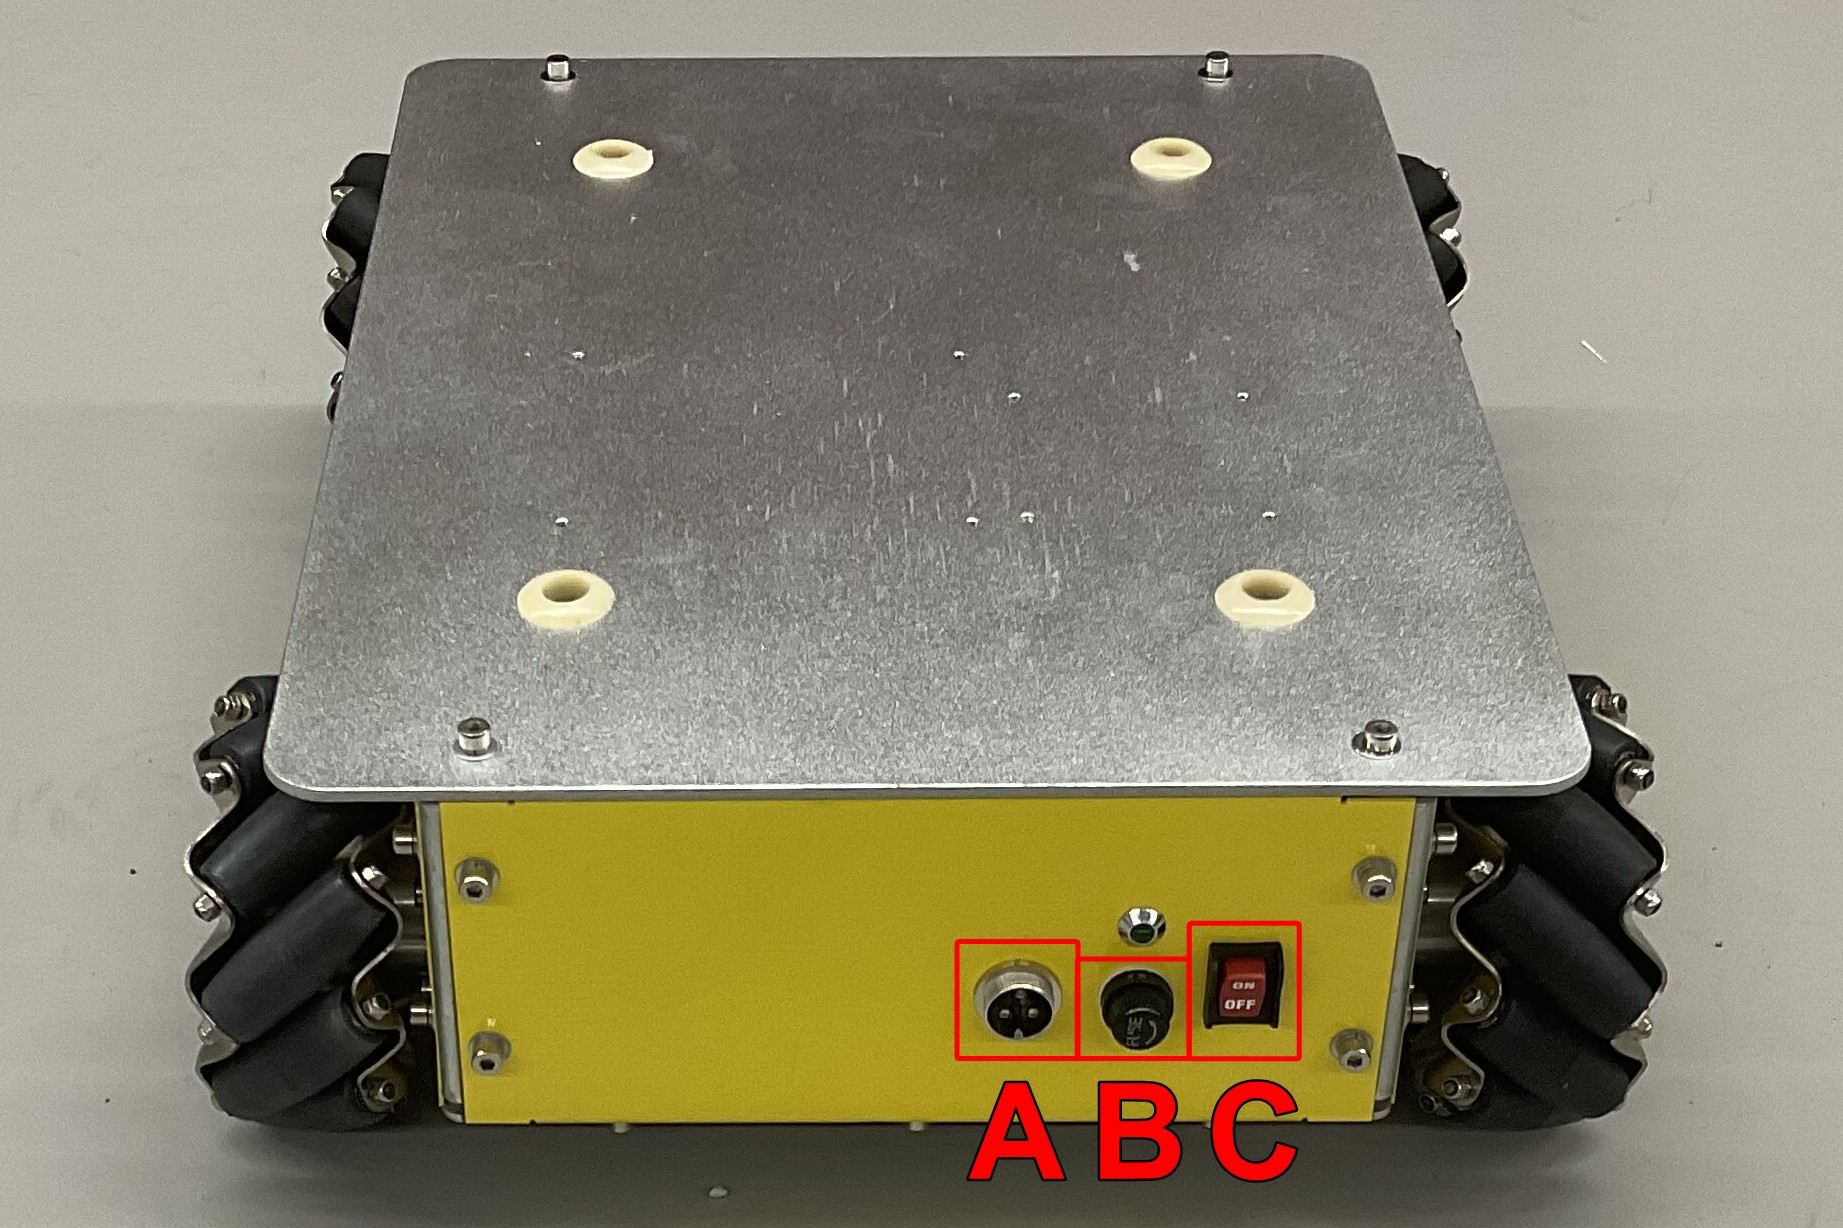
\includegraphics[width=0.4\columnwidth]{figs/hangfa-discovery-q2_original_annotated.jpg}
\caption{Original Hangfa Discovery Q2 mobile platform
(A: recharger socket; B: power fuse; C: power switch).}
\label{fig:hangfa:original}
\end{figure}

\subsection{Original platform}

The original Hangfa Discovery~Q2
is a small robot platform ($359\times 313.5\times 114$~mm
and 7~kg weight, with a 23 mm ground clearance) developed by
Hangfa Robotics\footnote{\label{note:hangfa}%
\url{https://www.hangfa-europe.com/}}.
This platform is a four-wheeled omnidirectional robot.
Consequently, the robot has holonomic kinematics,
allowing its linear and angular velocities to be decoupled from each other
(i.e., drive in any direction without requiring 
rotation)~\cite{sousa2024icarsc}.
The Discovery~Q2 also has a coaxial pendulum suspension
on its back wheels, enabling the four wheels to touch the ground
while helping reduce some vibration when passing through rough ground.

Furthermore, the robot is equipped with the
QMA10 mecanum wheels from Hangfa Robotics.
These wheels are 101.6~mm in diameter and 45.7~mm wide,
with a carbon steel hub, a 350~g weight, a 30~kg maximum load, and 10~rollers.
Each roller has rubber and two bearings to fix them to the wheel,
facilitating the platform to move smoothly and steadily.
The shaft of an outer body bearing block bears the wheel
in axial and radial load,
where the motor shaft is only used to transfer torque,
improving the robot's load capacity (rated at 20~kg).
Moreover, the DC motors are the
Faulhaber 2342 Original Equipment Manufacturer~(OEM) model,
with a 64:1 gear ratio and a
12~counts per revolution 5~V encoder with two channels at the motor shaft.
These motors are rated with a 12~V voltage, 1.1~A current, 11~W output power,
and 5800~Rotations Per Minute~(RPM) speed, with a 6800~RPM no-load speed.
As a result, the robot has a 0.65~m/s maximum translational and a
140º/s maximum rotation speed.

Regarding the electronics, the original robot
has a 12~V DC 10400~mAh Lithium-ion~(Li-ion) battery.
This battery allows more than 10~hours of autonomy,
with a 3~kg load, a moving speed of 0.5~m/s, and a 70\% moving rate.
The charger is $100\sim 240$~V AC with a DC output rated at 12.6~V~@~3.0~A.
Next, the IFB1205 board provides the 12~V and 5~V DC power buses
and makes Controller Area Network~(CAN) and RS232 interfaces
accessible to other modules.
The board also provides a 5~V~@~5~A DC output for external devices.
Moreover, the robot has a main power switch to turn ON/OFF
and a 10~A power fuse for electrical protection.

As for the motor drivers,
the IMDR4 module drives the four motors and provides closed-loop control.
This module implements the motion control algorithm of the
four omnidirectional wheels,
where the user can control the robot's linear and angular velocity
or the individual speed of the wheels.
The control is made through the CAN bus and RS232 interfaces.
However, the IMDR4 module does not provide data for wheeled odometry
to estimate the robot's pose through the 
robot's kinematic model and the displacement of the wheels.

The original platform provides a C\# Software Development Kit (SDK)
to communicate with the internal STM32F407 microcontroller.
The latter is part of the RHF407 development board.
The user may extend the platform by programming the RHF407 board,
connecting devices to the CAN bus,
or adding accessories such as a remote controller and laser sensors.

Still, the original platform has some drawbacks.
First, the Discovery~Q2 does not have a computing unit,
e.g., to run ROS-based nodes.
Next, wheeled odometry data is not available to the user.
The encoder signal of the motors could be derived to
another microcontroller, counting the pulses
based on the quadrature of dual channel encoders~\cite{sa2016mscthesis}.
However, this approach requires having two microcontrollers in the robot.
Also, the IMDR4 board does not have an interface
to change the internal closed-loop control.
Furthermore, only a 5~V~@~5~A DC external output is provided to the user,
limiting the possibilities of powering external 2D and 3D LiDARs,
or other equipment that may require more current or a different voltage level.
Lastly, the platform does not support natively 3D LiDAR or RGBD cameras.

\subsection{Electronics redesign}

So, this paper proposes a complete redesign of the
Discovery~Q2 platform's electronics.
\figref{fig:electronics} presents the proposed electronics layout,
which integrates custom 3D-printed components to accommodate all the
electronic devices,
simplifying the assembly and improving the organization.
Moreover, the 3D-printed structure features a two-level design.
The baseplate hosts the motor drivers (Cytron MD10C R3)
and a passive Battery Management System (BMS)
for 3S Lithium Polymer~(LiPo) batteries with a maximum current of 20~A.
Next, the upper level houses the microcontroller
(Arduino Mega 2560 with a proto shield to host encoders and 
motor drivers' connectors)
and a 5--30~V to 1.25--30~V DC/DC Buck-Boost Converter with a 
maximum current of 8~A.
Then, the battery (Tattu 10000~mAh 11.1~V 3S LiPo
with a 150~A maximum continuous discharge current)
and the electrical connectors (voltage and ground electrical buses)
are accessible to both the base and upper levels of the electronics structure.

\begin{figure}[t]
\centering
\subfloat[][]{\includegraphics[width=0.6\columnwidth]{figs/electronics_3d-framework_baseplate_annotated.jpg}%
\label{fig:electronics:baseplate}}
\linebreak
\subfloat[][]{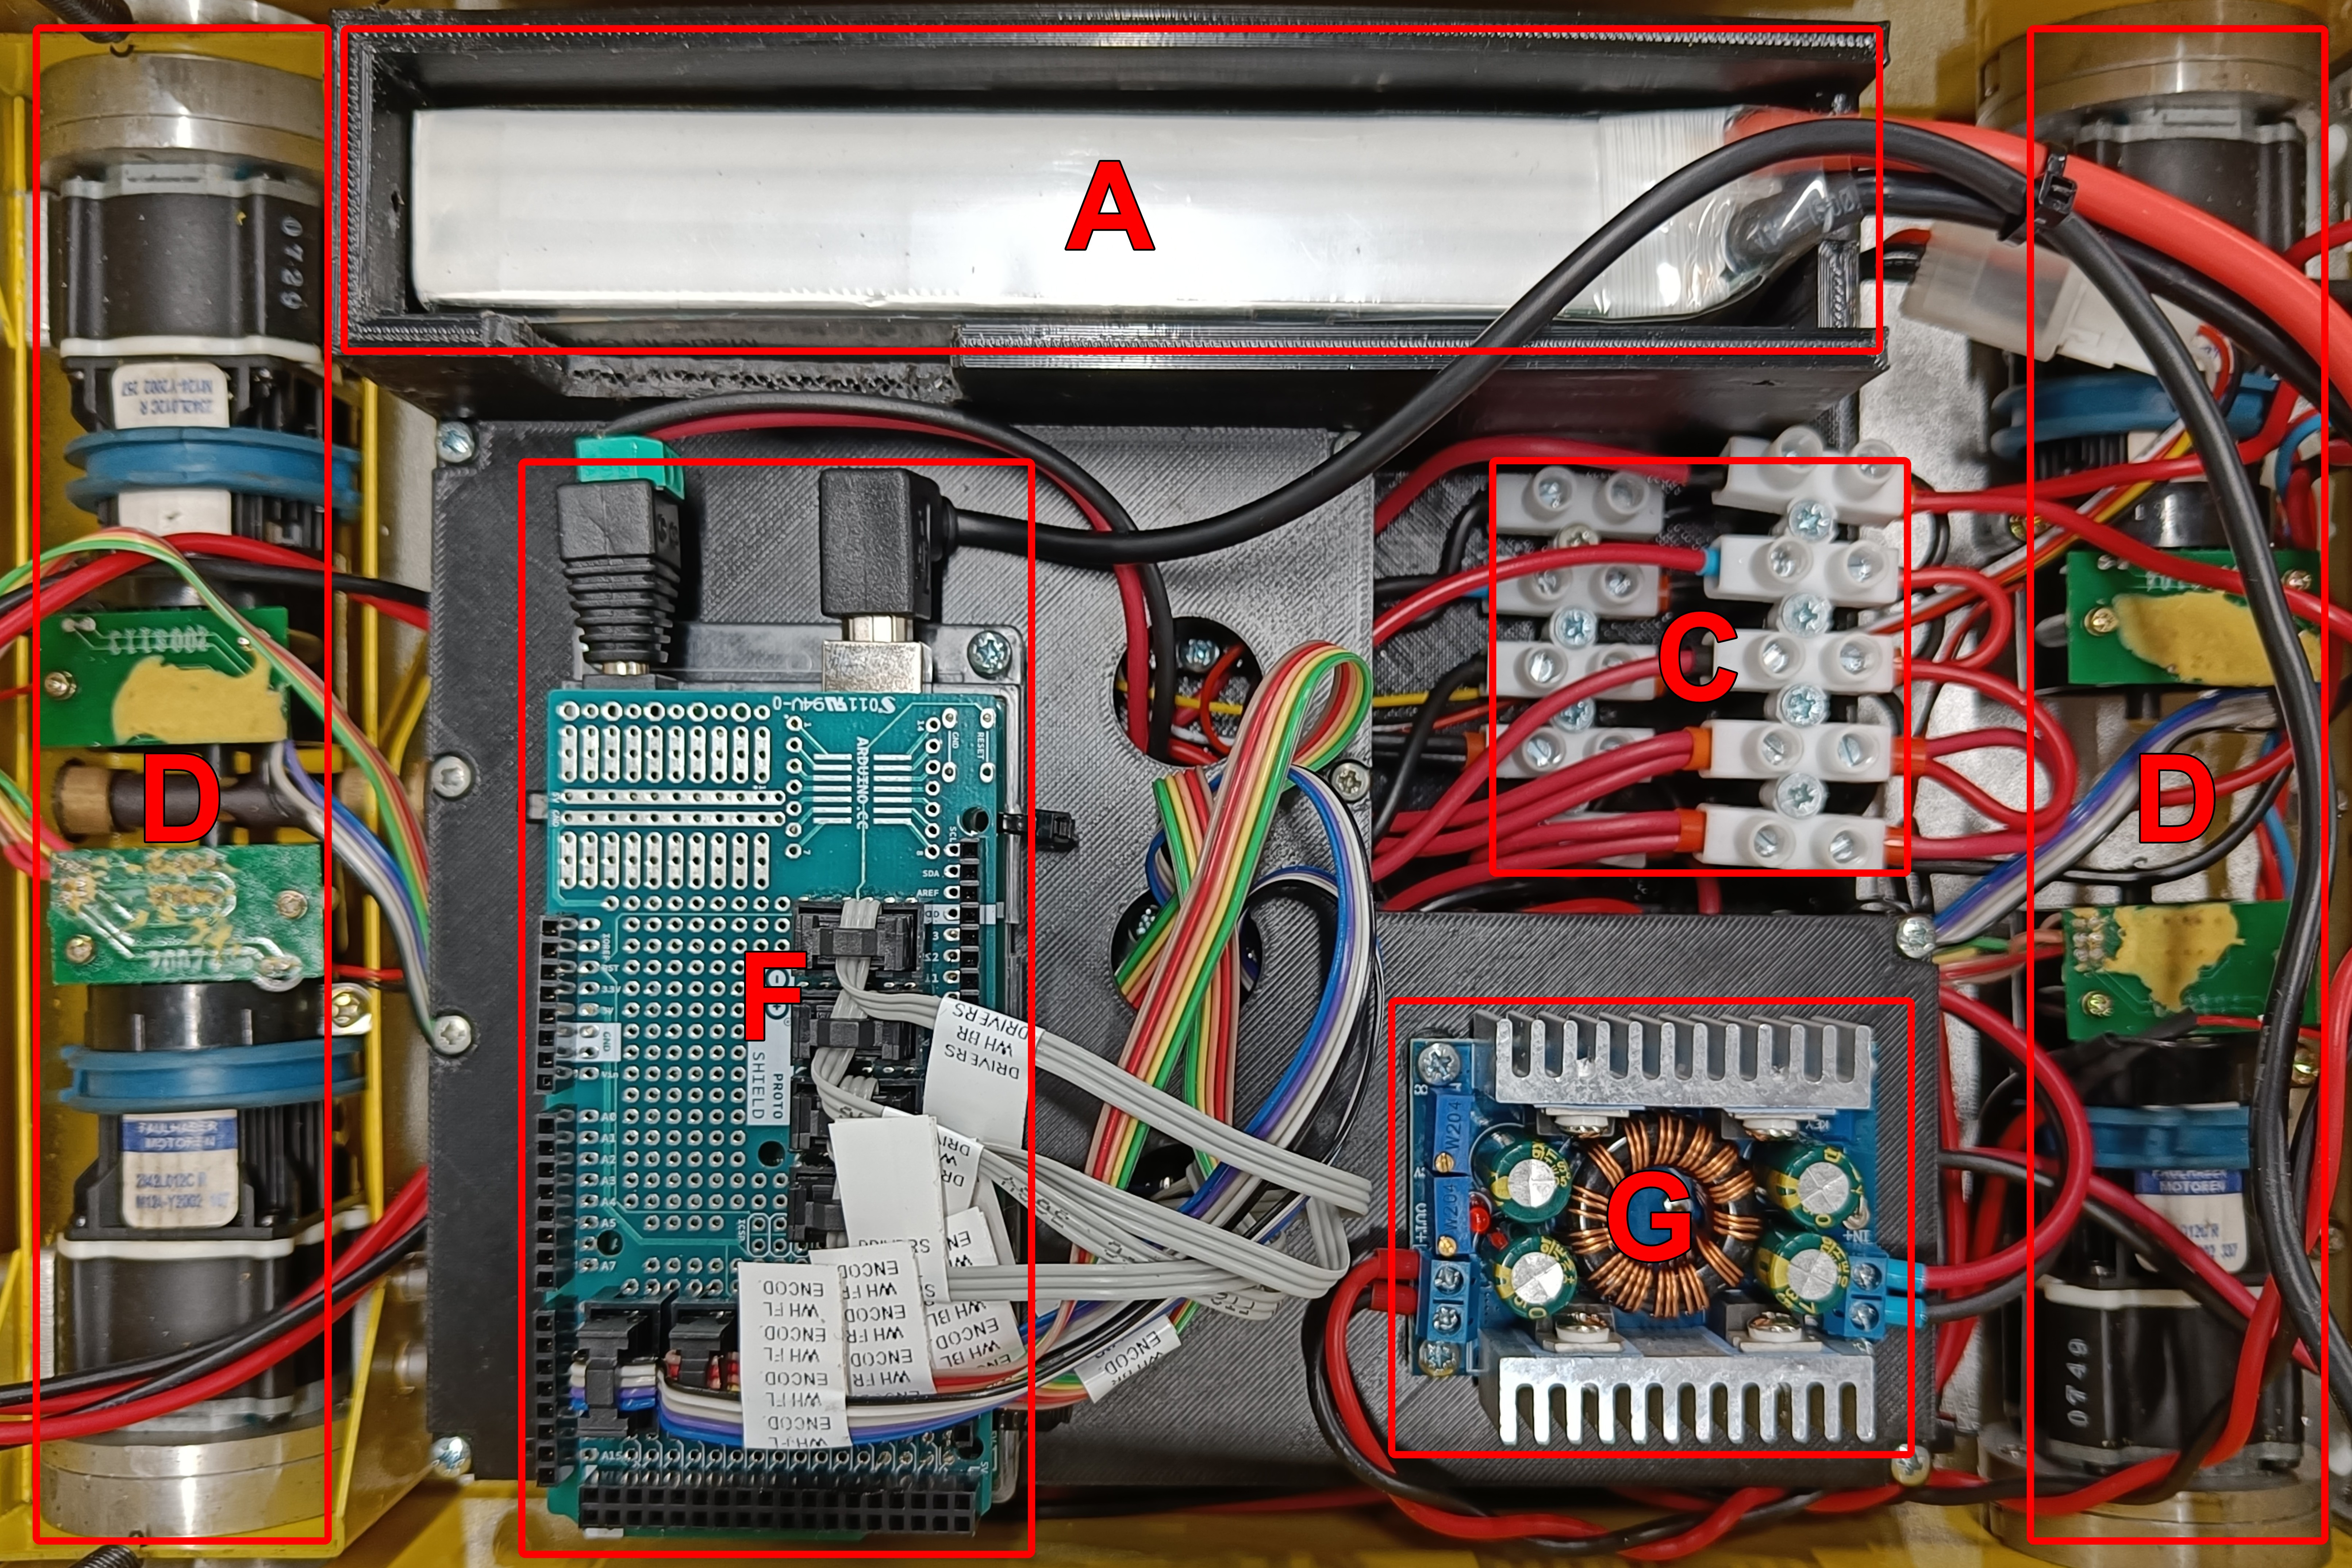
\includegraphics[width=0.6\columnwidth]{figs/electronics_3d-framework_1st-level_annotated.jpg}%
\label{fig:electronics:1st-level}}
\caption{Electronics redesign to integrate multimodal perception into
the Discovery~Q2 platform:
(a) baseplate;
(b) 1st level
(A: battery; B: BMS; C: voltage and ground electric buses; D: wheel motors;
E: motor drivers; F: microcontroller; G: DC/DC Buck-Boost converter).}
\label{fig:electronics}
\end{figure}

In terms of powering the robot,
the 3S battery output connector and its balance plug are directly connected
to the cell interface of the BMS (0~V, 3.7~V, 7.4~V, and 11.1~V).
The BMS's output is then connected to the
robot's ON/OFF switch and a new 20~A power fuse,
ensuring protected power delivery to all electronic components.
This configuration enables the BMS to passively 
maintain the battery cells' balance
during charging and discharging.
For regulated voltage, the DC/DC Buck-Boost converter is connected to the 
BMS output. This converter can provide
12~V or 24~V DC-regulated power supply voltages,
explicitly chosen for their compatibility with
all LiDAR sensors considered for the platform
(both in terms of voltage level and being regulated).
Ouster OS sensors are suitable for 12 and 24~V~DC nominal systems.
The voltage range of the Livox~Mid-360 (9--27~V) and the
RoboSense Helios~Series (9--32~V) is also compatible with 12 and 24~V~DC.
As for Velodyne Puck~Series, its voltage range is
9--18~V~DC, requiring to have the converter output to 12~V~DC.
Even if the users may have different requirements in terms of output voltage,
the converter has a wide voltage adjustment range (1.25--30~V).
Regarding recharging the platform,
the BMS has a recharging voltage between 12.6 and 13.0~V
and a maximum current of 10~A,
making it compatible with the original charger of 12.6~V~@~3.0~A from the Discovery Q2 platform.

As for the motors, each one is connected to a
single-channel motor driver MD10C~R3.
The platform's manual does not state the maximum current of the OEM Faulhaber~2342 motor,
only the 12~V and 1.1~A rated voltage and current, respectively.
Nevertheless, the maximum 13~A continuous and 30~A peak 
(for 10 seconds) currents
of MD10C~R3 should be adequate to drive the motors.
Next, the drivers are powered directly by the BMS,
in which the motor's 12~V rated voltage aligns with the
range of the 3S LiPo battery (approximately 9.6--12.6~V).
Finally, the Pulse-Width Modulation~(PWM)
and direction control inputs of the drivers
are linked to the Arduino Mega Proto Shield via 6-way
Insulation-Displacement Contact~(IDC) connectors,
consistent with those used for the motors' encoders.
This approach simplifies the interface for 
drivers and encoders by using a single connector type.

The microcontroller is also powered directly by the BMS output,
as its input voltage range of 6--20~V is compatible
with 3S LiPo batteries.
Instead of relying on the Arduino Mega's internal pull-up resistors
(20--50~k$\Omega$), external 3.3~k$\Omega$ pull-up resistors are soldered to the
channels A and B inputs of the four encoders on the 
microcontroller's proto shield
in order to reduce signal noise and improve
the quadrature between channels A and B.
These resistors are connected to the 5~V rail provided by the 
Arduino to form pull-up resistors.
The same 5~V rail also powers the motors' encoders.

In summary, the electronics redesign proposed in this paper
for the original Discovery~Q2 introduces several improvements
by enhancing its power capability and improving control flexibility.
Indeed, the maximum current increases from 10~A to 20~A.
Even though the official user manual does not clarify the maximum current
supported by the original Li-ion battery,
the 10~A value is based on the power fuse present previously in the platform.
Still, the 20~A is only limited by the BMS
(the newer battery supports a continuous discharge current up to 150~A),
allowing the user to upgrade to a 40~A BMS or even a higher current capacity.
This increase in power capability also enables additional external devices,
such as 2D/3D LiDAR systems.
Also, connecting encoders and PWM signals to the microcontroller
allows users to implement different closed-loop control architectures,
such as Proportional-Integrative (PI) controllers for 
angular speed control of the motors.

\subsection{Firmware}

The firmware on the revised platform is implemented on the
microcontroller Arduino Mega 2560.
This paper builds upon the firmware developed for the
\ifdefined\finalversion
Robot@Factory 4.0 competition~\cite{sousa2024icarsc}.
\else
\textit{Removed for blind revision}.
\fi
The firmware implements the same methodology for
processing the encoder signals
based on the quadrature inherent to two-channel encoders.
This approach accounts for the motor and the encoder's specifications,
including the 64:1 gear ratio on the motors
and the 12 counts per revolution resolution of the encoders
present on the original robot.
As a result, this configuration enables a resolution of
48 and 3072 pulses per revolution on the 
motors' shaft and at the wheels, respectively.
The latter resolution corresponds to an 
angular resolution of 0.117º/pulse at the wheel shaft.

Similarly, the firmware incorporates the serial communication protocol
based on the channels library used in the previous
\ifdefined\finalversion
work~\cite{sousa2024icarsc}.
\else
work~\textit{(Removed for blind revision)}.
\fi
This protocol defines the data exchange between
the microcontroller and an external computing unit.
Furthermore, the channels protocol defines a single compact message type:
the first byte specifies the data channel (type of information),
and the subsequent data packet represents the data value.
The latter is represented in binary (e.g., integer or float) or
ASCII (hexadecimal representation of the data value as characters),
corresponding to 4 and 8 bytes for the 
size of the data value on the package, respectively.
Thus, the firmware follows a similar channels configuration
from the previous work, communicating
the pulses count of the wheels' encoders (\texttt{g}--\texttt{j}),
interval time between control cycles (\texttt{k}),
reset signal (\texttt{r}),
reference speed of the four motors (\texttt{G}--\texttt{J}),
and the PWM value applied to the motors if needed (\texttt{K}).

% \begin{itemize}[nosep]
% \item Arduino Mega $\rightarrow$ External Computing Unit:
%   \begin{itemize}[nosep]
%   \item \texttt{g}: pulse count of the back-right wheel (ticks)
%   \item \texttt{h}: pulse count of the back-left wheel (ticks)
%   \item \texttt{i}: pulse count of the front-right wheel (ticks)
%   \item \texttt{j}: pulse count of the front-left wheel (ticks)
%   \item \texttt{k}: interval time between control cycles (us)
%   \item \texttt{r}: reset signal
%   \end{itemize}
% \item External Computing Unit $\rightarrow$ Arduino Mega:
%   \begin{itemize}[nosep]
%   \item \texttt{G}: reference speed of the back-right wheel (rad/s)
%   \item \texttt{H}: reference speed of the back-left wheel (rad/s)
%   \item \texttt{I}: reference speed of the front-right wheel (rad/s)
%   \item \texttt{J}: reference speed of the front-left wheel (rad/s)
%   \item \texttt{K}: PWM value of the motors:
%     \begin{itemize}[nosep]
%     \item (value $>>$ 24) \& 0x03: motor index (0..3)
%     \item (value) \& 0xFFFF: PWM value (0..max)
%     \end{itemize}
%   \end{itemize}
% \end{itemize}

Although this work adopts the same PI-based control system
for the wheels' angular speed control from the previous
\ifdefined\finalversion
work~\cite{sousa2024icarsc},
\else
work~\textit{(Removed for blind revision)},
\fi
this paper introduces improvements in PWM generation and code optimisations.
The
\ifdefined\finalversion
Robot@Factory framework
\else
\textit{Removed for blind revision}
\fi
uses the Adafruit Motor Shield v2
for the Arduino Mega to drive four motors.
The shield has limitations in terms of maximum current and switching frequency,
having a maximum of 1.2~A per motor
(with a maximum 3~A peak for a duration of around 20~ms),
close to the rated current of 1.1~A for the Faulhaber motors.
Furthermore, the shield's reliance on an internal PWM driver chip
and I2C bus communication for motor control results in a
maximum PWM frequency supported by the 
shield's library\footnote{\url{https://github.com/adafruit/Adafruit_Motor_Shield_V2_Library}}
of approximately 1.6~kHz. This frequency is within the audible range,
leading to undesired acoustic noises during operation.

Consequently, this paper adopts drivers that 
support external PWM signal generation
(MD10C~R3 supports up to 20~kHz switching frequency).
The PWM is generated from the microcontroller, using
\textit{TimerOne~\&~TimerThree}\footnote{\label{note:timers-lib}\url{https://www.pjrc.com/teensy/td_libs_TimerOne.html}}
libraries.
As a result, the proposed firmware achieves 
100~Hz for the closed-loop angular velocity speed control of the motors,
instead of 50~Hz on the previous
\ifdefined\finalversion
work~\cite{sousa2024icarsc},
\else
work~\textit{(Removed for blind revision)},
\fi
while not generating audible noise.
This improvement on the firmware loop rate leads to the odometry data
being available also at a 100~Hz.

\subsection{Computing unit \& networking}

The computing unit selected for the revised Hangfa Discovery Q2 platform
is the LattePanda 3~Delta Single Board Computer~(SBC),
illustrated in \figref{fig:sbc-networking}.
This SBC has the Intel Celeron N5105 quad-core processor with four threads,
a base clock of 2.00~GHz (boosting up to 2.90~GHz),
and a Thermal Design Power (TDP) of 10 W.
The processor includes an internal 
Intel UHD Graphics GPU with 24 execution units,
operating at 450--800~MHz, and supports up to three external monitors.
Moreover, the LattePanda 3~Delta features 8~GB of LPDDR4 RAM at 2933~MHz
and 64~GB of onboard eMMC storage.
The SBC also incorporates an M.2 PCIe 3.0 interface,
supporting an NVMe SSD to increase storage capacity and performance.
Indeed, in this paper, the Samsung 970 EVO Plus 250 GB NVMe SSD
has been added as the primary storage device
to improve both storage capacity and read/write speeds.

Regarding USB connectivity,
the LattePanda 3~Delta provides two USB 3.2 Gen 1 ports,
one USB 3.2 Gen 2 port (all Type-A),
and a USB Type-C port with Power Delivery~(PD),
which can power the SBC.
As for network connectivity,
the SBC supports WiFi~6 at 2.4/5~GHz, Bluetooth~5.2, and 2.5~Gbps Ethernet.
One advantage of the LattePanda 3~Delta is its x64-bit architecture,
offering enhanced compatibility with ROS 1 and ROS 2 environments
and open-source ROS-based packages,
compared to ARM alternatives such as Raspberry Pi boards.
Although the onboard ATMega~32U4
available in the SBC is not used as the microcontroller,
another advantage of the LattePanda 3~Delta
is having that microcontroller that could be used alongside the main processor.

\begin{figure}[t]
\centering
\includegraphics[width=0.6\columnwidth]{figs/sbc-and-networking_annotated.jpg}
\caption{LattePanda 3 Delta Single Board Computer (SBC) and the
networking solution for the revised platform
(A: Ethernet switch; B: computer battery;
C: LattePanda 3 Delta; D: WiFi antennas).}
\label{fig:sbc-networking}
\end{figure}

In terms of powering the SBC, the LattePanda 3~Delta offers three options.
The first is the LattePanda UPS~Hat, 
which utilises three 18650 Li-ion cells
and supports power delivery through Type-C~PD and 5.5~mm DC interfaces.
A key benefit of this solution is its support for the HID-UPS protocol,
enabling the operating system to recognise it as a battery device.
However, the overall battery capacity of the UPS~Hat would be
limited to the maximum capacity of one 18650 Li-ion cell, around 3600~mAh.
The second option powers the SBC with 12~V DC 
through the JST~PH2.0-4Pin connector.
This option is compatible with the DC/DC converter
integrated into the revised platform,
provided its output is regulated to 12~V.
However, relying on the converter may reduce the
overall current available for external devices
(LattePanda 3~Delta requires at least 2~A),
restrain the converter's output voltage to 12~V,
or even need an additional converter for external devices
if another voltage is needed such as 24~V~DC.

Thus, in this work, the SBC is powered
using the Xiaomi~Mi 50~W 20000~mAh power bank
via the USB Type-C PD interface.
A drawback is requiring an additional adapter to recharge the power bank.
Nevertheless, using a power bank
isolates the SBC electrically from other internal electronics and
increases the battery capacity compared to the UPS Hat,
depending on the power bank the user selects.
The SBC accepts PD-compliant devices at 15~V~@~3~A or 12~V~@~3~A.

As for the networking architecture,
the SBC provides wireless and Ethernet connectivity.
This paper proposes to use WiFi to
connect the SBC to networks available at the robot's deployment site.
This connection is facilitated by attaching
two Bingfu Dual Band WiFi Antennas to the robot's frame
(see \figref{fig:sbc-networking}) and connecting them to the
SBC's onboard Intel AX201 WiFi~6 wireless card.
Then, the 2.5~Gbps Ethernet port provides a
local network to connect sensors or other devices
to the robot by having an Ethernet switch.
The switches proposed for use in this paper are the
Brainboxes 5-Port 10/100~Mbps SW-005 or
1~Gbps SW-015 models,
both compatible with the revised platform regarding input power (5--30~V).



\section{Multimodal Perception Design \& Integration}

Integrating multimodal perception into the revised platform
involves mechanical sensor mounting and software integration
with the computing unit. First, the mechanical design proposed for
sensor fixation is presented, detailing the approach of using a bent
metal sheet and 3D-printed components. Then, the sensors are integrated
into the platform by leveraging the ROS compatibility
of the revised platform and the sensor drivers.

\subsection{Mechanical design \& sensors integration}

\begin{figure*}[t]
\centering
\subfloat[][]{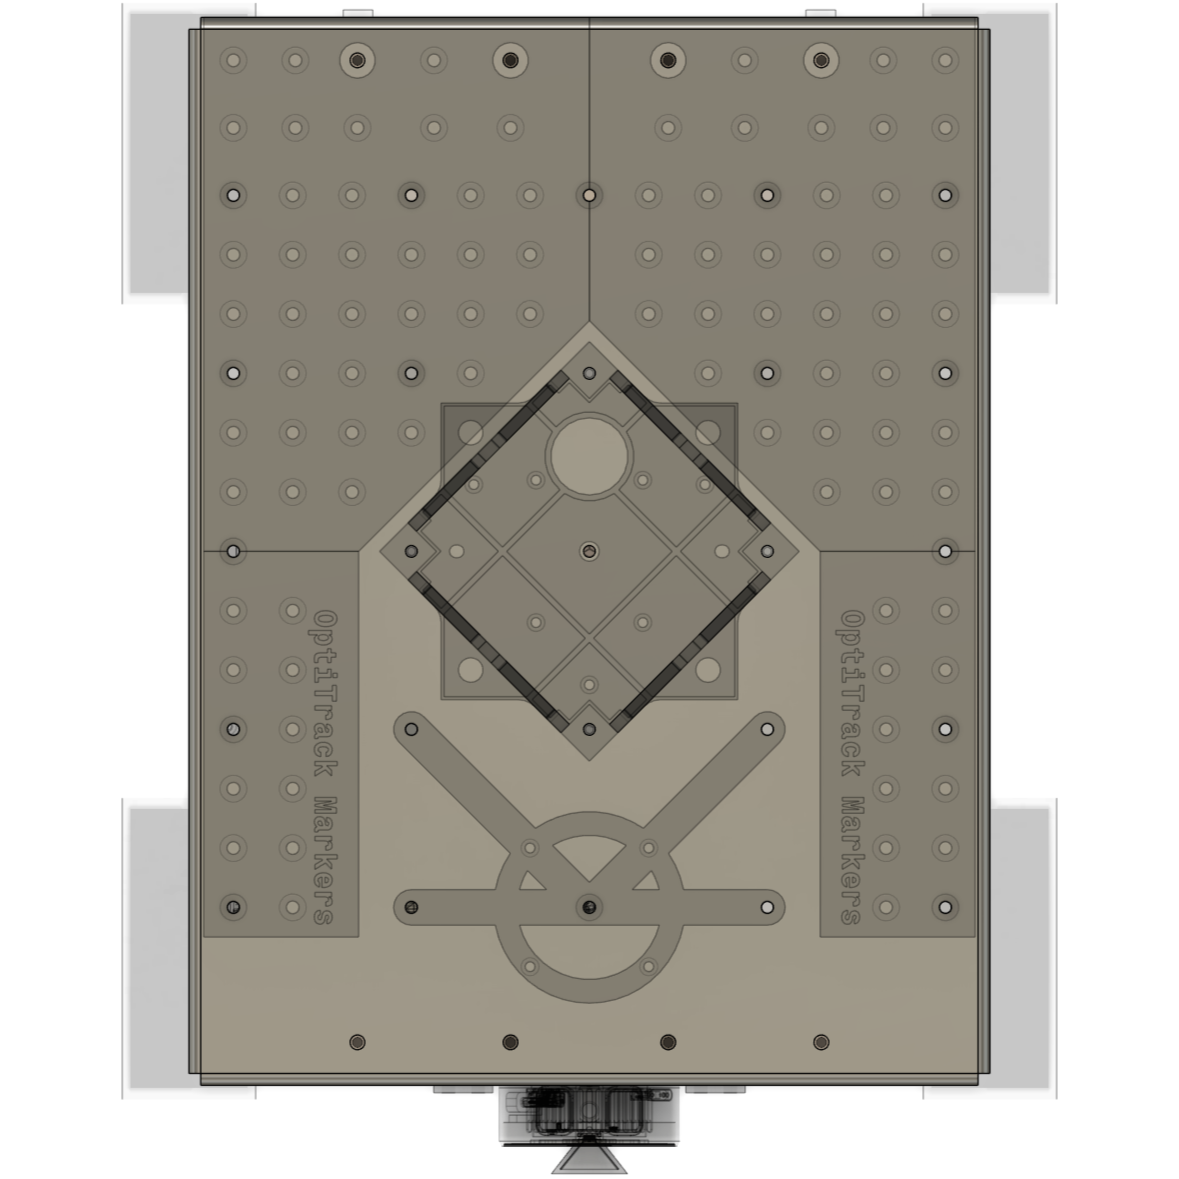
\includegraphics[width=0.225\textwidth]{figs/hangfa-discovery-q2_revised-platform_3d-model_photo_top_bend-metal-sheet_square.png}%
\label{fig:fusion-360:metal-sheet}}
\hspace{1em}
\subfloat[][]{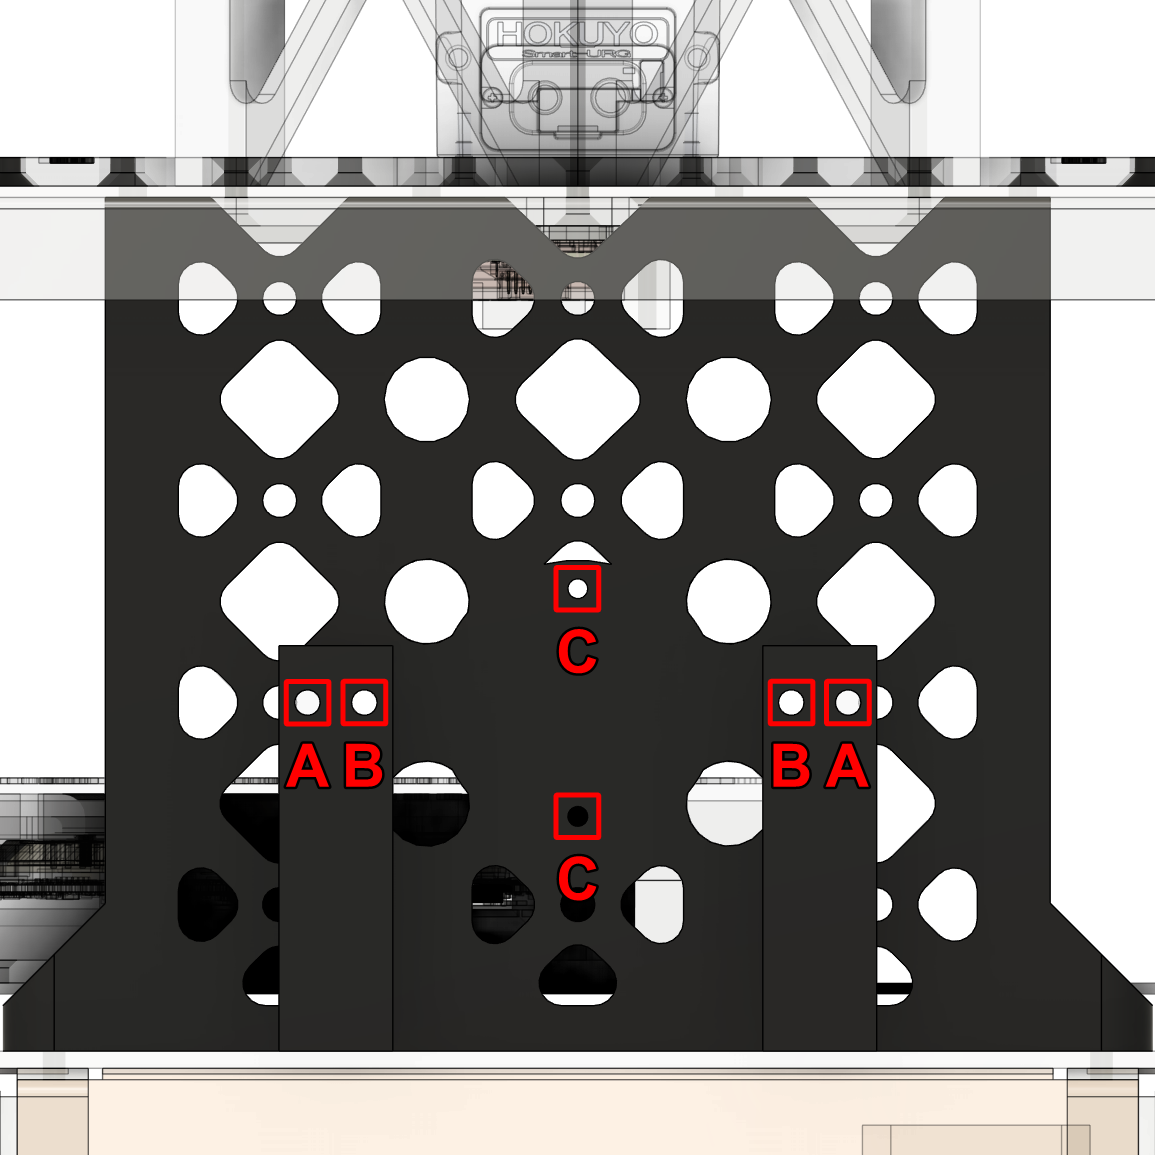
\includegraphics[width=0.225\textwidth]{figs/hangfa-discovery-q2_revised-platform_3d-model_photo_front_support-rgbd_square_annotated.png}%
\label{fig:fusion-360:rgbd}}
\hspace{1em}
\subfloat[][]{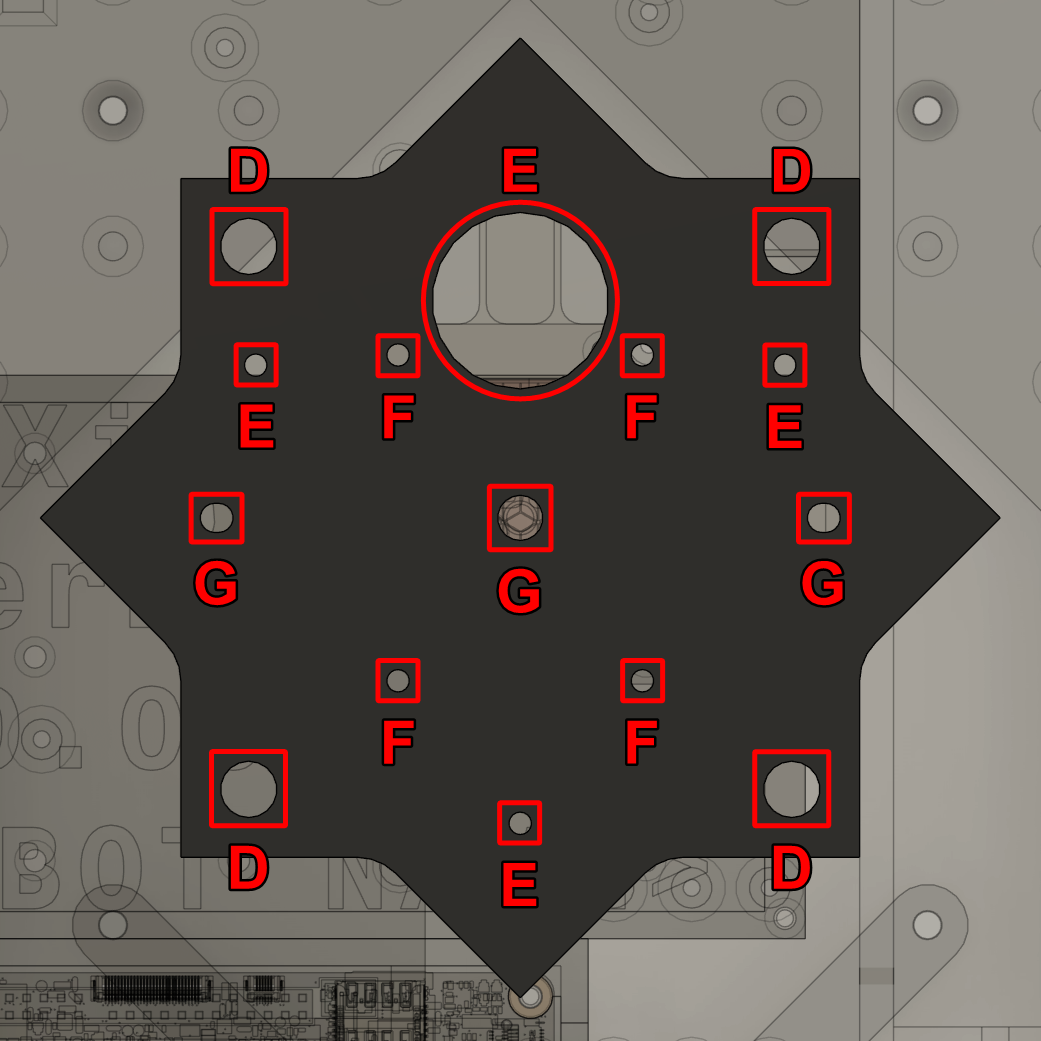
\includegraphics[width=0.225\textwidth]{figs/hangfa-discovery-q2_revised-platform_3d-model_photo_top_generic-support-lidar-3d_square_annotated.png}%
\label{fig:fusion-360:lidar-3d}}
\caption{3D model views on AutoDesk Fusion~360:
(a) top view of the bend metal sheet;
(b) front support of the metal sheet for RGBD cameras
(A: Intel RealSense~D455/455f/456;
B: OAK-D and OAD-D Pro Series;
C: Intel RealSense~L515);
(c) support on top of the metal sheet for LiDARs 3D
(D: Ouster OS sensors;
E: RoboSense Helios Series;
F: Livox Mid-360;
G: Velodyne Puck/VLP).}
\label{fig:fusion-360}
\end{figure*}

The mechanical design for integrating multimodal perception
into the revised Discovery~Q2 aims to facilitate the integration of
different sensors and enable the indexation of
sensor placement through CAD designs.
This indexation facilitates an initial estimation
for the sensors' extrinsic parameters.
As a result, a laser-cut bent metal sheet with evenly distributed M4 holes
is designed to host sensors such as 2D lasers, 3D LiDARs,
and possibly RGBD cameras (see \figref{fig:fusion-360:metal-sheet}).
The metal sheet is made of Aluminum AW~1050 with 2~mm thickness.
The bent shape on all sides increases the
overall stiffness of the sheet.
As for the holes, the laser cut process
used in this work can achieve a
0.1--0.2~mm precision for cutting the whole sheet and its holes.
% for cutting the whole sheet
% and its holes can achieve a 0.1--0.2~mm precision,
% according to
% Amorins \& Silva -- Indústria Metalomecânica\footnote{\label{note:amorins}%
% \url{https://amorinsesilva.pt/}}
% (company that machined and cut the metal sheet).
This tolerance allows a precise indexation of the sensors
compared to manually drilling the metal sheet.

Moreover, the M4 holes form a $5\times 5$ matrix
with a 60~mm spacing, covering an area of $240\times 240$~mm.
As a result, the outer dimensions of the final bent metal sheet
are $360\times 270$~mm, compared to the Discovery Q2's dimensions
of $359\times 313.5$~mm, avoiding exceeding significantly
the base footprint of the robot.
In order to secure the plate to the robot's frame,
eight M5 holes are positioned on the top surface of the metal sheet
(four at the front and four at the back).
These holes fixate the sheet to the 3D-printed PETG supports
shown in \figref{fig:hangfa:revised-platform} and \figref{fig:sbc-networking}.
These supports are specifically designed for the Discovery Q2 platform
to align with the four screws on the original top plate
(see \figref{fig:hangfa:original}).
The alignment provides the indexation of the bent metal sheet with respect to
the base.

In terms of sensors placement,
the ranging sensors (2D/3D LiDARs) are mounted on the bent metal sheet.
This placement design minimises obstructions
caused by the robot's body. As illustrated in
\figref{fig:hangfa:revised-platform} and \figref{fig:fusion-360},
2D laser scanners are positioned near the front of the metal sheet.
3D LiDARs are mounted at the centre in an elevated position
to avoid the sensor beams being obstructed by the robot's body.
Although a 360º 2D laser scanner may have obstructions
using the placement proposed in this paper,
those obstructions are due to the 3D LiDAR fixation support
and not to the robot's body.
Also, the 3D LiDAR support may be dismounted when not needed
or even retrieve a 360º 2D point cloud from the LiDAR itself.
RGBD cameras are placed on the front of the 3D-printed support
that fixates the bent metal sheet to the robot
(see \figref{fig:fusion-360:rgbd}).
This placement ensures an unobstructed Field Of View~(FOV)
to the front of the robot while avoiding stacking sensors on top of each other,
facilitating the design of the fixation supports. Nevertheless,
the platform users may place the sensors differently
on the metal sheet, leveraging the holes pattern to
index the sensors to the CAD designs.

Tables~\ref{tab:specs:rgbd}--\ref{tab:specs:3D-lidars}
present specification comparisons of
the sensors considered in this paper
for multimodal perception integration into the revised platform.
The three RGBD cameras (Intel RealSense D455/L515, and OAK-D Pro)
do not require separated DC power, only need an USB connection to the SBC.
Furthermore, three 2D laser scanners (LD-19, RPLIDAR S2, and YDLIDAR X4)
are also powered directly through the USB connection.
In contrast, the Hokuyo UST-10LX sensor
is connected to the DC/DC converter
and the data transmission is provided through Ethernet.
As for 3D LiDARs, similar to the Hokuyo sensor, the four LiDARs
(Livox Mid-360, Ouster OS1~64 Rev~C, and RoboSense RS-HELIOS-5515)
are connected to the DC/DC converter and the Ethernet switch.

\begin{table}[!t]
\renewcommand{\arraystretch}{1.15}
\setlength{\tabcolsep}{0.275em}
\caption{Specification Comparison of the RGBD Sensors
Intel RealSense D455, Intel RealSense L515, and OAK-D Pro}
\label{tab:specs:rgbd}
\centering
\begin{tabular}{l l c c c}
\hline
\bfseries Specs&&\bfseries RS D455&\bfseries RS L515&\bfseries OAK-D Pro\\
\hline
Color & H/VFOV (º) & 90º/65º & 70º/43º & 69º/55º\\
      & Res. (px)  & $1280\times 800$ & $1920\times 1080$ & $4056\times 3040$\\
      & Rate (fps) & 30 & 30 & 60\\
      % & Shutter    & global & rolling & rolling\\
\hline
Depth & Type       & active stereo & LiDAR & active stereo\\
      & H/VFOV (º) & 87º/58º & 70º/55º & 80º/55º\\
      & Res. (px)  & 1280x720 & 1024x768 & 1280x800\\
      & Rate (fps) & 90 & 30 & 120\\
      & Range (m)  & 0.6--6 & 0.25--9 & 0.7--12\\
\hline
\end{tabular}
\end{table}

\begin{table}[!t]
\renewcommand{\arraystretch}{1.15}
\setlength{\tabcolsep}{0.275em}
\caption{Specification Comparison of the 2D Laser Scanners
Hokuyo UST-10LX, LD-19, RPLIDAR S2, and YDLIDAR X4}
\label{tab:specs:2D-lasers}
\centering
\begin{tabular}{l c c c c}
\hline
\bfseries Specs & \bfseries UST-10LX & \bfseries LD-19 &
\bfseries RPLIDAR S2 & \bfseries X4\\
\hline
FOV/Res. (º) & 270º/0.125º & 360º/0.8º & 360º/0.1125º & 360º/0.432--0.864º\\
Type         & ToF & ToF & ToF & Triangulation\\
Rate (Hz)    & 40 & $\sim 10$ & $\sim 10$ & $\sim 10$\\
Range (m)    & 0.06--10 & 0.02--12 & 0.05--30 & 0.12--10\\
\hline
\end{tabular}
\end{table}

\begin{table}[!t]
\renewcommand{\arraystretch}{1.15}
\setlength{\tabcolsep}{0.275em}
\caption{Specification Comparison of the 3D LiDARs
Livox Mid-360, Ouster OS1~64 Rev~C,
RoboSense RS-HELIOS-5515, and Velodyne VLP-16}
\label{tab:specs:3D-lidars}
\centering
\begin{tabular}{l c c c c}
\hline
\bfseries Specs & \bfseries Mid-360 & \bfseries OS1~64 &
\bfseries HELIOS-5515 & \bfseries VLP-16\\
\hline 
H/VFOV (º)  & 360º/59º & 360º/45º & 360º/70º & 360º/20º\\
HRes. (º)   & -- & 0.176/0.352/0.703º & 0.1/0.2/0.4º & 0.1--0.4º\\
VRes. (º)   & -- & 0.71º & $\le 1.33$º & 1.33º\\
VRange (º)  & -7--+52º & -22.5--+22.5º & -55--+15º & -10--+10º\\
VType       & non-uniform & uniform & non-uniform & uniform\\
\#channels  & -- & 64 & 32 & 16\\
Rate (Hz)   & 10 & 10/20 & 5/10/20 & 5--20\\
Range (m)   & 0.1--70 & 0.3--120 & 0.2--150 & 100\\
\hline
\end{tabular}
\end{table}

Overall, the RGB cameras, 2D lasers, and LiDARs considered in this paper
offer diversity in terms of sensor resolution,
depth and ranging estimation types
-- active stereoscopy versus LiDAR on RGBD cameras,
Time-of-Flight~(ToF) versus triangulation on 2D lasers --,
FOV resolution and range
(including uniform versus non-uniform vertical FOVs on 3D LiDARs),
and acquisition rate.
This diversity allows the test of 2D/3D SLAM and object detection algorithms,
among others, with different multimodal characteristics
while having initial estimation for the sensors' extrinsic parameters.
Still, other sensors may be used as long as
their power and communication requirements are compatible with the
platform, only requiring adapting or even design
new 3D-printed fixation supports.

\subsection{ROS integration}

A ROS driver was developed for the revised platform based on a
USB serial connection for the SBC to communicate with the
firmware running on the microcontroller. The driver publishes the
data from the wheel encoders and subscribes to the reference angular speed
for the motors. Then, a ROS node computes the wheel odometry based on
the kinematics of a four-wheeled omnidirectional robot~\cite{sousa2022jint}.
Both the ROS driver and the odometry estimation node are compatible with
ROS 1 and ROS 2 to improve the platform's usability.

Since all the sensors considered in this work have ROS-compatible drivers,
the data can be published directly in ROS.
Integrating the sensors and the revised platform in ROS enables the
data acquisition throughout the environment and execution of
algorithms that leverage multimodal perception capabilities,
either open-source or developed by the user.

% \subsection{External tracking system}

% 4 tracking spheres, one on each wheel.
% other spheres are put on top of the robot.

% 1. OptiTrack used to align the rigid body with the 4 tracking spheres on each wheel,
% aligned with the robot's odometry coordinate referencial.
% 2. Add spheres as contraints to the rigid body
% 3. remove the wheel spheres from the body to avoid adding error upon robot motion



%%%%%%%%%%%%%%%%%%%%%%%%%%%%%%%%%%%%%%%%%%%%%%%%%%%%%%%%%%%%%%%%%%%%%%%%%%%%%%%%



% \section{Experimental Evaluation}\label{sec:exp}
% Repeat the main focus/objective with one(!) sentence starting with:
% The main focus of this work is a  .....
% Explain the reader that the experiments with support all claims
%   (same list as in the intro!) starting the paragraph with:
% Our experiments are designed to show the capabilities of our method and to
% support our key claims, which are:
% %
% (i)~...,
% %
% (ii)~...,
% %
% (iii)~..., and
% %
% (iv)~....
% We furthermore provide comparisons to a popular method for ... as
% proposed in~\cite{stachniss2005aaai}.  We perform the evaluations on own
% datasets as well as on publicly available ones.  Throughout all these
% experiments, we set the key parameter of our approach to $X=1$ as this
% provided the best performance as shown in \figref{fig:parameval}.
% If needed (and only then!) say also a few words about the
%   experimental setup, the datasets, and used parameters. You can use
%   an own subsection if you want to put the focus on that but often that is
%   not needed.
% Note 1: It MUST be always crystal clear (a) WHY an experiment is
%   there (e.g., to support a claim, to show that the approaches useful
%   for real word systems, to show the performance, or to provide a
%   baseline comparison), (b) WHAT it wants to show (which
%   claim/property exactly), and (c) HOW it aims at showing this. This
%   is ESSENTIAL for a good evaluation. Think about when BEFORE
%   designing an experiment.
% Note 2: Start with the most important/impressive experiment
%   first. Make this a key story of the paper. Keep the order of the
%   claims, i.e., re-order claims in the intro/before if needed.
%
% \subsection{Performance}
% Start EVERY experiment with a similar start as the following
%   sentence, explaining in the first sentence why you present the
%   experiment and the claim it aims at supporting.
%% First experiment - most impressive, important or the most important
%% claim supporting experiments comes first.
% The first experiment is designed to show the performance of our
% approach and to support the claim that it is well-suited for ...
% \begin{figure}[t]
%   \centering
%  \includegraphics[width=0.99\columnwidth]{pics/motivation}
%   \caption{A caption that makes you understand the image easily.}
%   \label{fig:parameval}
% \end{figure}
%% Second experiment - could be a comparison to a baseline methods,
%% quality analysis or similar
% The second experiment is to support the claim that our approach is ...
%
% \subsection{Runtime}
%% Runtime experiment - it is often one of the last experiments unless
%% online processing/speed is the key contribution
% The next set of experiments is designed to support the claim that our
% approach runs fast enough to support online processing on the robot in
% real time. We, therefore, tested our approach on ...
% \tabref{tab:speed} summarizes the runtime results for .....  The
% numbers support our third (check!) claim, namely that the computations
% can be executed fast and in an online fashion.  On a mobile i5 CPU, we
% achieve average frame rates of XXX\,Hz-XXX\,Hz depending on ... and
% XXX\,Hz-XXX\,Hz on an i7 desktop computer.
% \begin{table}
% \caption{Average runtime and std.~dev.}
% \centering
% {\footnotesize
% \begin{tabular}{|c|c|c|}
% \hline
% XXXX & mobile & desktop \\
%  & i5 CPU 2.2\,GHz & i7 CPU 3.5 GHz\\
% \hline
% configA & 2.4\,ms~$\pm$~0.5\,ms~$\approx$~416\,Hz & 1.5\,ms~$\pm$~0.2\,ms~$\approx$~667\,Hz \\
% configB & 4.4\,ms~$\pm$~1.2\,ms~$\approx$~227\,Hz & 2.6\,ms~$\pm$~0.5\,ms~$\approx$~385\,Hz \\
% configC & 8.6\,ms~$\pm$~2.6\,ms~$\approx$~116\,Hz & 4.7\,ms~$\pm$~1.2\,ms~$\approx$~212\,Hz \\
% \hline
% \end{tabular}
% }
% \label{tab:speed}
% \end{table}
%
% \subsection{XXX Analysis}
% Finally, we aim at supporting our claim that ...
% Briefly summarize the evaluation and what follows with approx. 2
%   sentences.
% In summary, our evaluation suggests that our method
% provides competitive ... At the same time, our method is fast enough
% for online processing and has small memory demands. Thus, we supported
% all our claims with this experimental evaluation.

\section{Experimental Tests}

\begin{figure*}[t]
\centering
\subfloat[][]{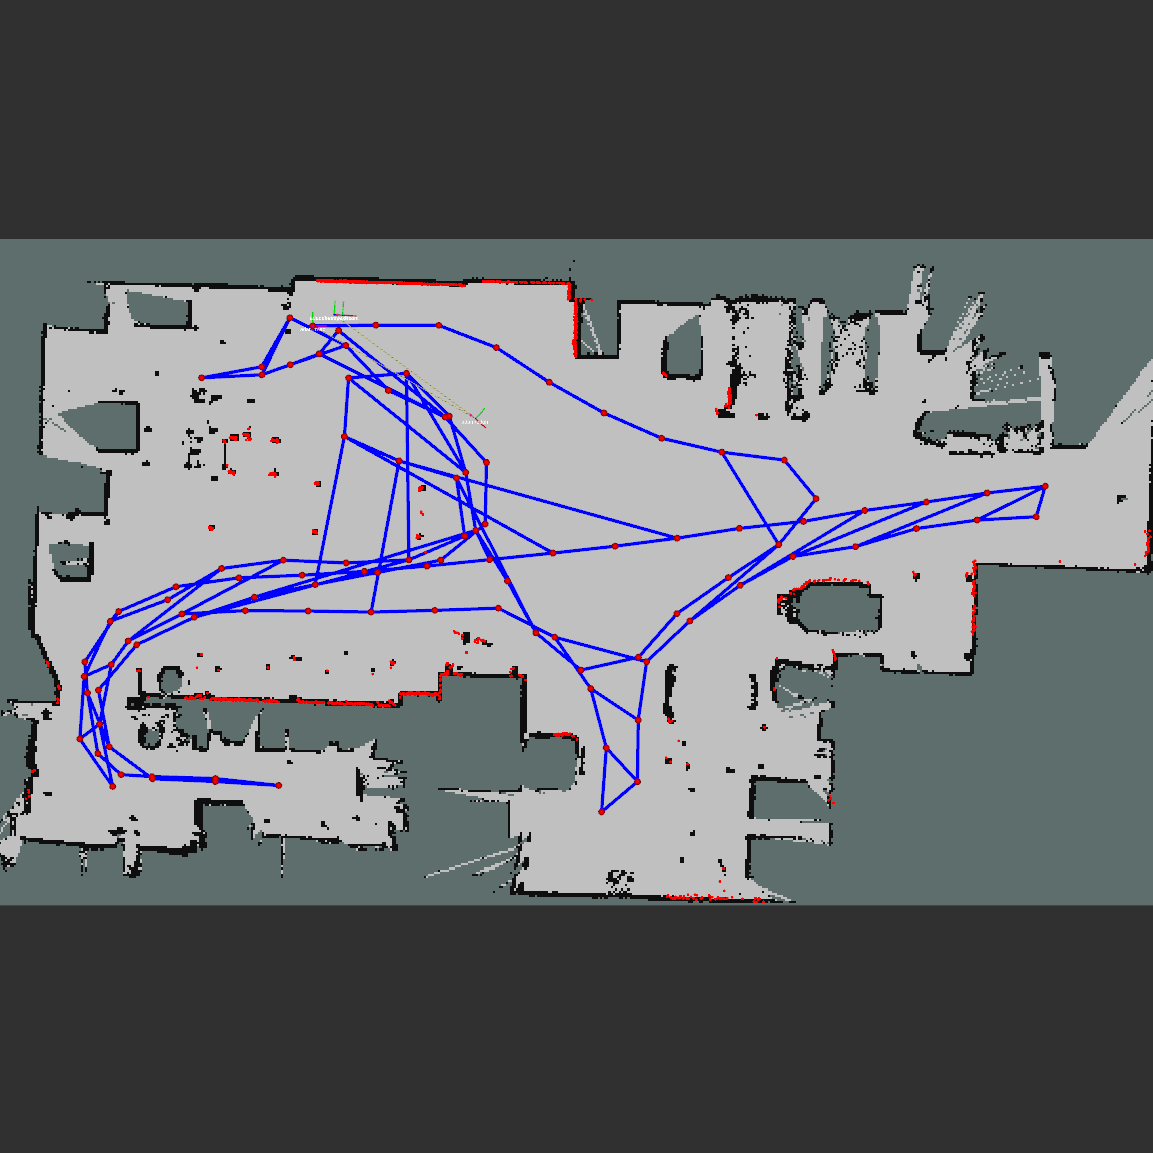
\includegraphics[height=0.3\textwidth]{figs/results_slam-2d.png}%
\label{fig:results:slam-2d}}
\hspace{1em}
\subfloat[][]{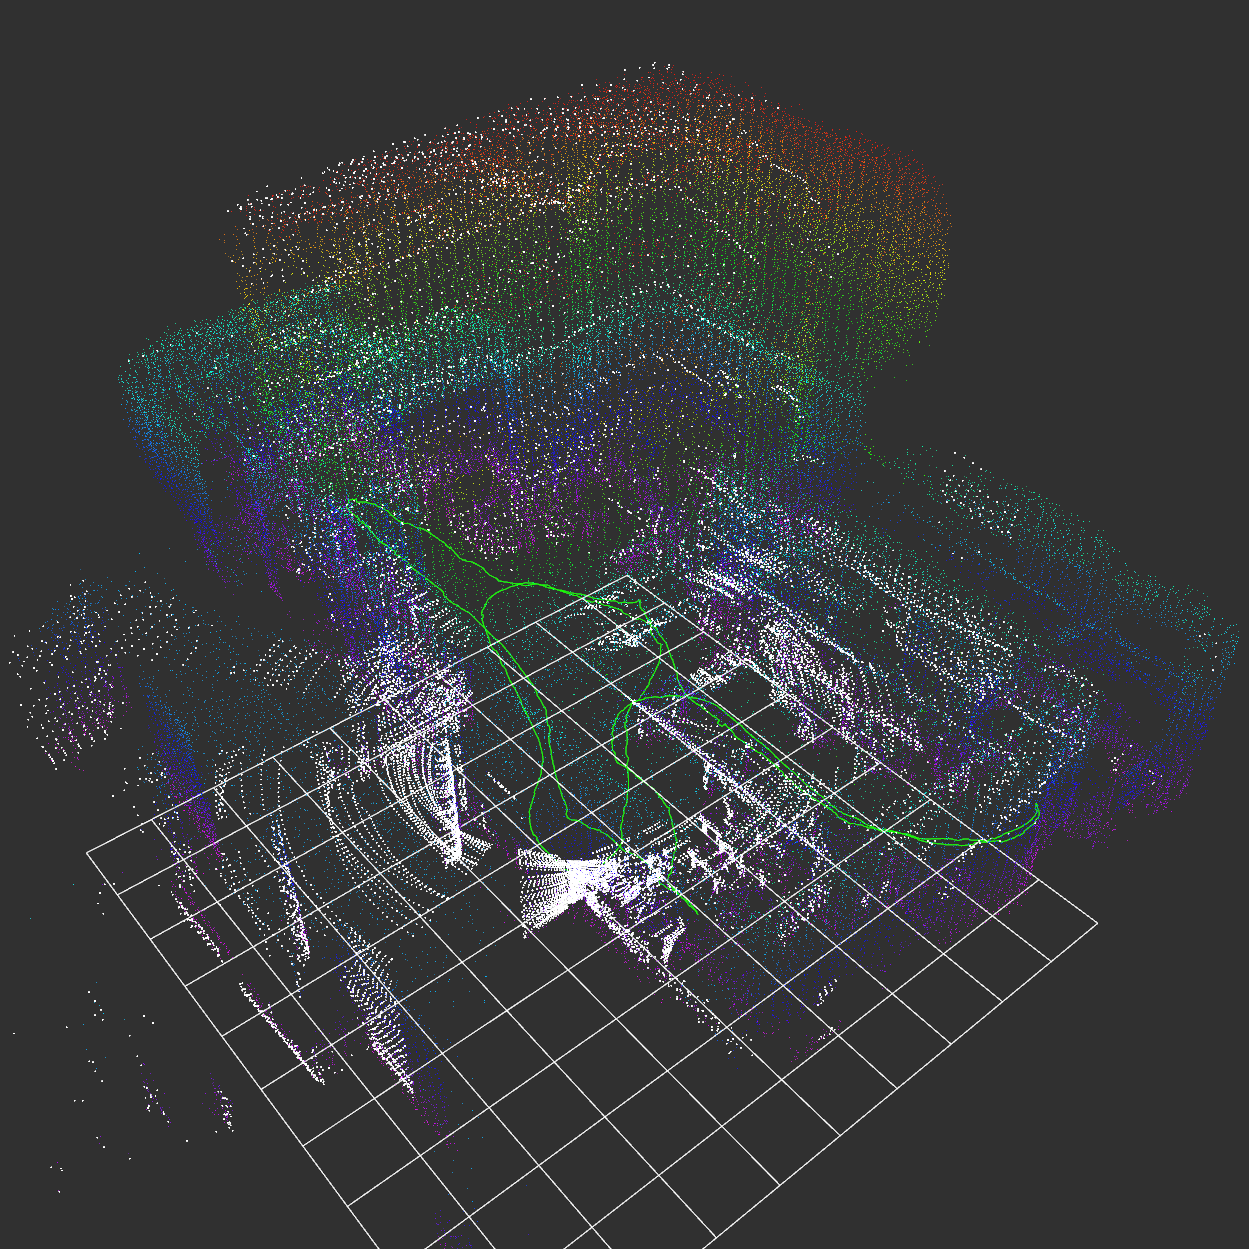
\includegraphics[height=0.3\textwidth]{figs/results_slam-3d.png}%
\label{fig:results:slam-3d}}
\hspace{1em}
\subfloat[][]{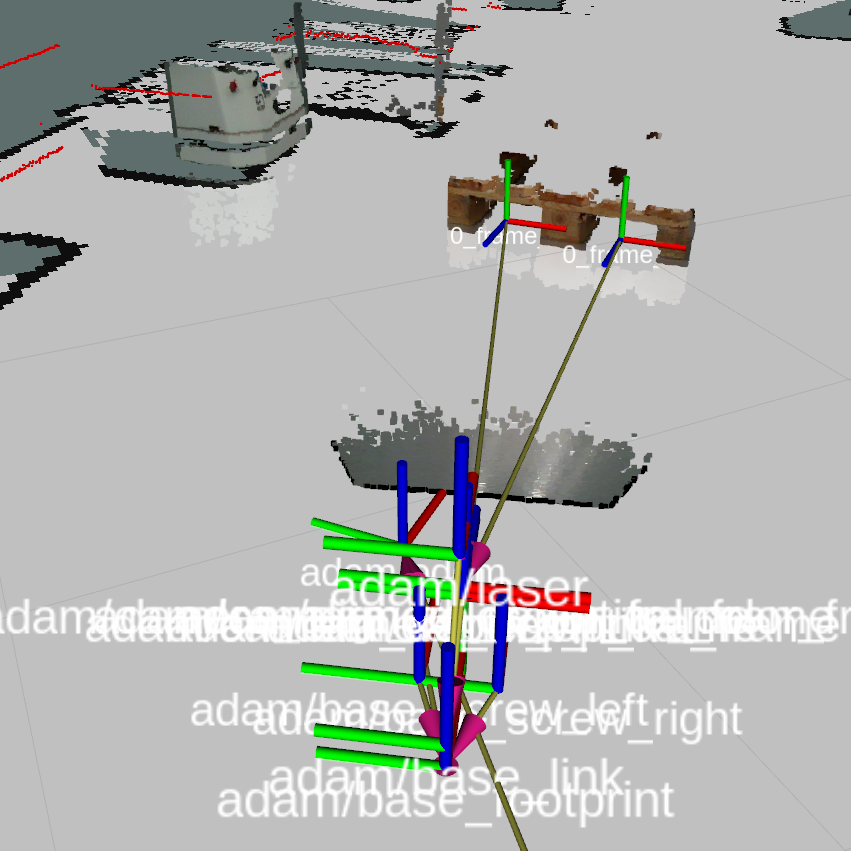
\includegraphics[height=0.3\textwidth]{figs/results_pallet-detection.png}%
\label{fig:results:pallet-detection}}
\caption{Experimental tests of the revised platform
with multimodal perception:
(a) 2D SLAM~\cite{macenski2021joss}
with wheel odometry and 2D laser scanner (Hokuyo UST-10LX);
(b) 3D SLAM~\cite{aguiar2023vineslam}
with wheel odometry and 3D LiDAR (Livox Mid-360);
(c) pallet pocket detection~\cite{caldana2024robot}
with 2D localisation~\cite{sobreira2019jint} and
RGBD perception (Intel RealSense L515).}
\label{fig:results}
\end{figure*}

% EXPERIMENTS CONDITIONS
% >>>>> LOCALISATION 2D
% - online
% - average rate of pose publication: odom > map 50Hz (SLAM Toolbox)
%                                     base > odom 100Hz (platform)
% - throttle_scans          : 1
% - transform_publish_period: 0.02 (still, no throttling)
%   (considering hokuyo at 40Hz...)
% >>>>> SLAM 3D WITH 3D LIDAR LIVOX
% - online
% - average rate of pose publication: 
% - n_particles: (not sure if highly dependent on #particles..., no rviz)
%   - 300: ~6-7Hz wo/ rviz (mid-360 @ 10 Hz)
%   - 200: ~6.5Hz
% - n_particles: (not sure if highly dependent on #particles..., no rviz)
%   - 300: 3Hz (rs-helios-5515 @ 5Hz)
% - doe the algorithm tries to process all scans when moving? yes...
% >>>>> PALLET POCKET PERCEPTION
% - offline processing (rosbag record of 2D localisation with RGBD perception)

The experimental evaluation of the proposed multimodal perception integration
into a ground mobile platform focused on
testing various robot perception applications.
\figref{fig:results} presents the experimental results with the
revised Discovery~Q2 platform. First, the platform executes online 2D~SLAM
using wheel odometry and 2D laser with the
SLAM Toolbox algorithm\cite{macenski2021joss}. With the latter configured to
skip only one scan, publishing the robot's pose at 50~Hz, and considering the
Hokuyo UST-10LX's rate of 40~Hz, the onboard SBC on the platform performed
2D~SLAM without throttling.
The second experiment executes 3D~SLAM using wheel odometry and 3D~LiDAR data
with the VineSLAM~\cite{aguiar2023vineslam} stack configured to 300~particles.
Using the Livox Mid-360 sensor, the onboard computer achieved an online SLAM
processing rate of approximately 7~Hz with a sensor rate of 10~Hz.
When using the RoboSense RS-HELIOS-5515, the online execution rate decreases to
approximately 3~Hz, possibly due to this sensor's higher data output
than the Mid-360 (576000~pts/s in single return mode versus 200000 pts/s,
respectively).

As for the third test, a multimodal perception application
is tested offline for pallet pocket estimation~\cite{caldana2024robot}
with 2D~localisation~\cite{sobreira2019jint}.
The data recording subscribed to all topics, including the ones from the
2D~localisation system and the Intel RealSense~L515
(set to $640\times480$~px resolution and 6~Hz and 30~Hz for RGB and depth data,
respectively). The offline processing demonstrates another application
of the proposed multimodal system in this paper:
gathering multimodal data and processing it offline for
research and development. Still, a possible alternative to run the algorithm
online could be using the LattePanda~Sigma SBC (12-core, 16-thread Intel~Core
i5-1340P processor and 32~GB of RAM). This SBC is also compatible with power
bank charging. However, the power bank must be upgraded to
support at least 90~W~@~20~V.
Videos from the experiments presented in this paper and additional tests
are available
\ifdefined\finalversion%
online\footnote{\href{https://www.youtube.com/playlist?list=PLvp8fJUEPxYSkKsOrCN5FzjuhhSfVgSuR}{https://www.youtube.com/playlist?\\list=PLvp8fJUEPxYSkKsOrCN5FzjuhhSfVgSuR}}.
\else%
online\footnote{\url{https://drive.google.com/drive/folders/1nZxhxqZdQJgYg-4uHu1dXiSMQd8ktrSC?usp=sharing}}.
\fi

% BMS            : 20 A max (also electrical fuse)
% OEM Motors     : 1.1A rated current >>> 4.4A drive motors
% MD10C R3       : no information on current...
% DC/DC Converter: typical ~90% efficiency rate, 8A max
% Ethernet switch:  1.1W = 0.092A@12VDC, 0.046A@24VDC (SW-005)
%                   3.6W = 0.300A@12VDC, 0.150A@24VDC (SW-015)
% 2D Laser       : 0.150A@24VDC (UST-10LX)
% 3D LiDAR       :  6.5W (Mid-360)
%                  23.0W = 0.958A@24VDC (OS-61)
%                  12.0W (RS-HELIOS-5515)
%                   8.0W (VLP-16)
%
% TOTAL CURRENT:
% DC/DC OUTPUT: 0.958A + 0.150A + 0.150A = 1.258A @ 24VDC OUTPUT
% DC/DC INPUT : 12VDC, 3.145A @ 80% efficiency (though typical 90%)
%
% 
%
% TOTAL PLATFORM: 4.4A + 3.145A = 7.545A >>> 10Ah / 7.545A = 1h20min approx
% (NOTE considering the motors at rated current, which is not thinkable)



%%%%%%%%%%%%%%%%%%%%%%%%%%%%%%%%%%%%%%%%%%%%%%%%%%%%%%%%%%%%%%%%%%%%%%%%%%%%%%%%



\section{Conclusions and Future Work}\label{sec:conclusion}

% In this paper, we presented novel approach to....
% Our approach operates ...  Our method exploits ...
% This allows us to successfully ...
% We implemented and evaluated our approach on different datasets
% and provided comparisons to other existing techniques and supported
% all claims made in this paper. The experiments suggest that ...
%
% Future work only if it makes sense
% Future work: Use only if applicable -- but if so, use the following sentence to start:
%
%Despite these encouraging results, there is further space for
%improvements. For example, ...

In conclusion, this paper proposes a comprehensive methodology to
integrate multimodal perception into a ground mobile robot
leveraging 3D printing, laser cutting, and bending metal sheet
fabrication processes. The methodology includes mechanical, electronics,
firmware, computation and networking architecture aspects while
providing an initial estimation of the extrinsic sensor parameters
from CAD designs. While the integration focused on adapting the
Hangfa Discovery~Q2 platform for multimodal perception, the revision made
to the original robot can be extended to similar platforms or even adjusted
to meet voltage, power, computation, and sensorisation requirements.
The multimodal perception system is demonstrated in real-world experiments
through online and offline data processing, showcasing its capability in
applications such as 2D SLAM, 3D SLAM, and pallet pocket detection.
All electronics documentation, mechanical designs,
along with the code developed in the scope of this paper,
are open-source and made available in a public repository\footref{note:repo}.
For future work, the platform will be used and tested further for research and
development, SLAM benchmarking, sensor calibration algorithms,
and RGBD perception in industrial applications.





%%%%%%%%%%%%%%%%%%%%%%%%%%%%%%%%%%%%%%%%%%%%%%%%%%%%%%%%%%%%%%%%%%%%%%%%%%%%%%%%



\section*{Acknowledgements}\label{sec:acknowledge}

The authors would like to acknowledge all the support from the
\ifdefined\finalversion%
5dpo Robotics Team\footnote{\url{https://5dpo.github.io/}},
\else%
\textit{Removed for blind revision},
\fi%
Amorins \& Silva\footnote{\url{https://amorinsesilva.pt/}}
% Amorins \& Silva\footref{note:amorins}
for their expertise in machining bent metal sheets,
Hangfa Robotics\footref{note:hangfa}
for their support related to the Discovery Q2 platform,
and the LattePanda Team\footnote{\url{https://www.lattepanda.com/}}
for their sponsorship and technical support.



%%%%%%%%%%%%%%%%%%%%%%%%%%%%%%%%%%%%%%%%%%%%%%%%%%%%%%%%%%%%%%%%%%%%%%%%%%%%%%%%



% All new citations should go to references.bib. The file glorified.bib
% should go be the one from the ipb server. After paper or related work has
% been written merge the entries from references.bib to glorified.bib ON THE
% SERVER, replace the glorified.bib in this repository and empty the
% references.bib

\bibliographystyle{IEEEtran}
\bibliography{references}

% \printbibliography

\end{document}

%%%%%%%%%%%%%%%%%%%%%%%%%%%%%%%%%%%%%%%%%%%%%%%%%%%%%%%%%%%%%%%%%%%%%%%%%%%%%%%%
%% NOTES ON PAPER WRITING
%
% Rename the paper.tex file into your paper name. Use the BibTeX key policy
% (see below)
%
% Use a Spell Checker with US English as spelling language
%
% Use Academic Writing Check: https://github.com/devd/Academic-Writing-Check
%
% Use GIT for version control. Use our gitlab sever!
%
% Make sure your Makefile is working correctly and compiles the documents
%
% All images go to the subfolder figs and reviews into the reviews folder
%
% Make sure the source files for images are in the figs folder as well
% (unless they are huge)
%%%%%%%%%%%%%%%%%%%%%%%%%%%%%%%%%%%%%%%%%%%%%%%%%%%%%%%%%%%%%%%%%%%%%%%%%%%%%%%%


%%%%%%%%%%%%%%%%%%%%%%%%%%%%%%%%%%%%%%%%%%%%%%%%%%%%%%%%%%%%%%%%%%%%%%%%%%%%%%%%
%% NOTES ON BIB ENTRIES
%
% Bibtex Key Policy
%
%    All in lower case
%    Use the key structure:
%        <lastnamefirstauthor><4 digit year><conference/journal><extra>
%    Use <extra>:
%        only to disambiguate: - first chars of the first 4 words f the title
%    Examples: stachniss2008icra, stachniss2008icraws, stachniss2008icra-adhc
%    Use the BibTeX key also at the filename for the paper, e.g.,
%    stachniss2008icra.pdf
%
% Bibtex Entries
%
%    Use strings for conferences and journal name in order to keep obtain
%    consistent entries
%    Use the identical abbreviations for conference name, e.g.,
%    "Proc. of the IEEE Int. Conf. on Robotics and Automation (ICRA)"
%    Avoid adding the location in addition to the city or street of the
%    conference.
%    Use doi for the official document on the publisher webpage.
%    Abbreviate the first name of the authors, e.g., C. Stachniss instead of
%    Cyrill Stachniss
%    In case of a first name and a middle name, use no space between them, e.g.,
%    C.J. Stachniss
%%%%%%%%%%%%%%%%%%%%%%%%%%%%%%%%%%%%%%%%%%%%%%%%%%%%%%%%%%%%%%%%%%%%%%%%%%%%%%%%
